% =====================================================================
%  Complejidad estructural y dificultad predictiva en la competencia M4
%  Version extendida para revista — agosto 2026
%
%  Requiere en el preambulo:
%     \usepackage{booktabs}   \usepackage{graphicx}
%     \usepackage{amsmath}    \usepackage{siunitx}   (opcional)
%     \usepackage[table]{xcolor}  (opcional, para el sombreado)
%
%  Las figuras van en  ./figuras/  (PDF vectorial, generadas por
%  generar_figuras.py). Subirlas a Overleaf en esa carpeta.
% =====================================================================

\title{Hasta dónde permite decidir la estructura de una serie,\\
       y por qué ahí se detiene\\
       \large Selección y combinación de modelos sobre las 100{,}000 series\\
       de la competencia M4}

\author{Jorge Andres Pe\~na Araya\thanks{Autor de contacto:
        \texttt{jorgeandrespena@icloud.com}} \and Esther Segura P\'erez}
% ---------------------------------------------------------------------
%  MARCA DE VERSION -- borrar las dos lineas de \version y el \\ que la
%  precede en \date antes de enviar a la revista.
%  Subir el numero en CADA subida a Overleaf, y usar el mismo texto en la
%  etiqueta del historial. Es lo que permite saber, abriendo el PDF, si se
%  esta mirando la ultima version: el conteo de paginas y el titulo no
%  distinguen entre versiones consecutivas.
% ---------------------------------------------------------------------
\newcommand{\versionborrador}{v9 \textperiodcentered{} 31 de octubre de 2026}

\date{Universidad Nacional Aut\'onoma de M\'exico (UNAM), Ciudad de M\'exico\\[2pt]
      {\small\ttfamily\versionborrador}}

% babel-spanish convierte el punto decimal a coma DENTRO de modo
% matematico, de modo que $0.411$ sale "0,411" y un 0.895 escrito en
% texto plano sale "0.895". El documento mezclaba las dos formas segun
% como se hubiera escrito cada numero. \decimalpoint las unifica en punto.
\decimalpoint

% Colocacion de flotantes: por defecto LaTeX manda a pagina propia cualquier
% figura que ocupe mas de la mitad del alto, lo que aqui dejaba tres paginas
% practicamente vacias. Estos valores le permiten acompanar figuras grandes
% con texto sin forzar nada.
% El espacio por omision alrededor de cada flotante (12 pt) deja, sumado sobre
% los veintitantos cuadros y figuras, casi una pagina de aire.
\setlength{\floatsep}{8pt plus 2pt minus 2pt}
\setlength{\textfloatsep}{10pt plus 2pt minus 2pt}
\setlength{\intextsep}{8pt plus 2pt minus 2pt}
\renewcommand{\topfraction}{0.9}
\renewcommand{\bottomfraction}{0.8}
\renewcommand{\textfraction}{0.07}
\renewcommand{\floatpagefraction}{0.8}
\setcounter{topnumber}{3}
\setcounter{bottomnumber}{2}
\setcounter{totalnumber}{4}

\maketitle

% ---------------------------------------------------------------------
\begin{abstract}
\noindent
¿Hasta qué punto las propiedades estructurales de una serie de tiempo permiten decidir
cómo pronosticarla? Es la premisa del pronóstico por características, y este trabajo la
somete a prueba sobre las 100{,}000 series de la competencia M4 para medir hasta dónde
llega. La respuesta es afirmativa y acotada: \textbf{la estructura sí permite decidir, de
manera estadísticamente sólida, pero el margen que recupera es pequeño, el límite no
proviene del instrumento y su causa es identificable.}

El instrumento es un \emph{índice de complejidad estructural}, el negativo de la primera
componente principal de 29 descriptores, en la línea de los espacios de instancias
\cite{kang2017} pero orientado a decidir y no a visualizar. Correlaciona con el error del
pronóstico ingenuo ($r=0.411$; $n=96{,}891$) y separa cuartiles cuyo error medio crece por
un factor de 3.29, aunque su poder discriminante depende con fuerza de la frecuencia.
Sobre una muestra estratificada de 5{,}773 series se evalúan 28 métodos bajo la métrica
oficial OWA y se comparan políticas en 30 particiones. Asignar modelo por frecuencia y
estrato mejora el OWA de $0.9140$ a $0.8835$ en las 30 ($p=1.9\times10^{-9}$), con dos
estratos como granularidad óptima: la misma cardinalidad ---no la misma frontera--- que un
análisis de conglomerados había hallado por criterios internos.

El techo aparece al medir cuánto recupera. Entre el modelo fijo y un oráculo retrospectivo
que elige el mejor método en cada serie ($0.923$ contra $0.542$), la regla recorre el
10.5\,\%; la fracción restante mezcla lo que las características no capturan con el error
que ningún candidato podía evitar, y acota por arriba lo que queda por ganar en lugar de
medir señal desaprovechada. Lo que delimita el alcance del instrumento es una comparación
interna: la mejor política sobre los 29 atributos recorre el 15.0\,\%, de modo que todo
ese aparato compra diecisiete milésimas de OWA sobre un escalar con dos estratos y deja
sin recuperar el mismo 85\,\%. La causa es medible: en el 76\,\%
de las series la arquitectura neuronal ganadora cambia solo al variar la semilla, y la
variante que clasifica el modelo ganador y le cree queda en $1.493$, peor que no enrutar
---no por ese ruido, según se muestra, sino por minimizar la pérdida equivocada---.
Repetido sobre M3 con los pronósticos publicados de 22 métodos, el techo se sostiene y
empeora ---allí queda sin recuperar el 93\,\%---, pero el margen del enrutamiento cae del
10.5\,\% al 1.9\,\%: lo gobierna la heterogeneidad del banco y no la de las series.

Ante una colección hay, sin embargo, dos decisiones y no una: qué método asignar a cada
serie y cuántos combinar. Medidas sobre los mismos datos con un \emph{bootstrap} que
remuestrea series, ambas ganancias son significativas y de magnitud comparable ---combinar
$+0.0267$ con intervalo $[+0.0143,\ +0.0393]$, estratificar $+0.0214$ con
$[+0.0110,\ +0.0328]$--- y su diferencia no lo es. La literatura por características
atiende casi solo a la primera, y lo que gobierna la segunda no es la estructura de las
series sino la dispersión de calidad del banco: con candidatos parejos combinar gana, y al
incorporar N-BEATS \cite{oreshkin2020} la conclusión se invierte en cada frecuencia donde
ese modelo domina, bajo un mismo mecanismo ---promediar cancela sesgos entre componentes
comparables y arrastra al mejor cuando uno domina---. El aporte del índice es máximo al
seleccionar ($+0.0215$) y se diluye al combinar hasta dejar de distinguirse de cero a
partir de tres modelos: la caracterización estructural resulta útil donde la política
elige, y no en los tamaños de conjunto que mejor rinden. Un resultado más modesto que el
que la premisa prometía y el que los datos sostienen.

\vspace{2mm}\noindent
\textbf{Palabras clave:} series de tiempo; competencia M4; características
estructurales; combinación de pronósticos; selección de modelos; análisis de
componentes principales; clustering; OWA; reproducibilidad.
\end{abstract}


% =====================================================================
\section{Introducción}
% =====================================================================

El pronóstico de series de tiempo es una actividad central en ingeniería industrial,
economía, energía y manufactura, y en entornos productivos el problema rara vez consiste
en pronosticar una serie: son miles ---una cadena de suministro con decenas de miles de
referencias, una red eléctrica que mide por subestación, una plataforma de comercio con un
histórico por producto---. Quien enfrenta esa escala no se pregunta cuál es el mejor
modelo, sino cuál para cuál serie.

Es una pregunta incómoda, porque no se puede responder probando. Ajustar decenas de
métodos a cien mil series es caro, y al terminar uno sabe cuál ganó en cada caso pero no
por qué, ni qué hacer con la serie siguiente. De ahí el atractivo de una idea sencilla: si
las series se pudieran describir por su forma ---cuánta tendencia, cuánta estacionalidad,
cuánta irregularidad--- tal vez esa descripción bastaría para anticipar qué método les
conviene, antes de ajustar ninguno. La competencia M4 \cite{makridakis2020} es el lugar
natural para ponerla a prueba: 100{,}000 series reales en seis frecuencias, de anual a
horaria, cuya heterogeneidad es a la vez su valor y su dificultad, porque una serie anual
de 13 observaciones y una horaria de 900 no admiten el mismo tratamiento.

Este trabajo construye esa descripción ---un índice de complejidad estructural sobre 29
descriptores--- y después hace lo que la literatura suele dar por supuesto: la pone a
decidir y mide cuánto rinde.

Rinde. Enrutar por estructura mejora de manera consistente sobre asignar modelo solo por
frecuencia, y gana en las treinta particiones evaluadas. Pero rinde poco. Entre el modelo
fijo y el oráculo que acierta el mejor método en cada serie queda un hueco grande, y el
enrutamiento recorre menos de su décima parte. Lo que convierte eso en un resultado y no
en una decepción es el control: un meta-aprendiz con los 29 atributos completos y un
regresor por modelo recorre prácticamente lo mismo. El techo no es del índice. La
información que haría falta para elegir bien existe ---el oráculo la tiene--- pero no
está en la forma de las series.

¿Por qué no está? Porque la etiqueta que habría que aprender no se queda quieta. Al
reentrenar las mismas redes sobre las mismas series cambiando únicamente la semilla de
inicialización, el modelo ganador cambia en tres de cada cuatro series. Ninguna
caracterización puede aprender a predecir algo que se mueve solo.

Ese diagnóstico abrió una pregunta que no estaba en la hipótesis de partida. Si elegir un
modelo es tan frágil, quizá el problema esté en elegir. Ante una colección hay
\emph{dos} decisiones, no una: qué método asignar a cada serie, y si conviene quedarse
con uno o promediar varios. La literatura de pronóstico por características se ocupa casi
solo de la primera. Medidas ambas en la misma escala, sobre los mismos datos y el mismo
protocolo, \textbf{la segunda pesa más}.

Y dentro de ese hallazgo hay otro. Cuál de las dos estrategias conviene no depende
tampoco de la estructura de las series, sino de algo bastante más simple: qué tan parejo
es el conjunto de modelos del que uno dispone. Si ninguno despega del resto, promediar
gana, porque los errores se cancelan entre sí. Si hay uno claramente superior ---y una
red global moderna entrenada sobre decenas de miles de series lo es--- promediar lo
arrastra hacia abajo y conviene quedarse con él. Es el mismo mecanismo que la literatura
de combinación describe desde sus orígenes; lo que se aporta aquí es medirlo sobre una
misma colección con un mismo protocolo, y mostrar que el régimen cambia de una frecuencia
a otra.

La caracterización estructural tampoco queda fuera de juego, pero su utilidad se
concentra donde menos se la esperaba: es máxima cuando la política \emph{elige} un modelo
y se diluye al combinar, hasta dejar de ser detectable con tres o más. Es menos de lo que
la premisa prometía, y es lo que los datos sostienen.

Las contribuciones son seis:

\begin{enumerate}
\item Una \textbf{prueba de utilidad y no solo de correlación} para la caracterización
      estructural: un experimento de enrutamiento con validación fuera de muestra en el
      que asignar modelo según frecuencia y estrato de complejidad supera a asignarlo
      solo por frecuencia en las 30 particiones evaluadas. La granularidad óptima ---dos
      estratos--- coincide con la cardinalidad que el análisis de conglomerados había
      identificado por criterios internos, aunque no con su frontera: las dos particiones
      concuerdan en el 70.1\,\% de las series y el conglomerado minoritario queda
      íntegramente contenido en el estrato de complejidad alta. Repetido sobre M3 con los
      pronósticos publicados de 22 métodos y el índice transferido sin reajuste, el
      experimento conserva el signo pero cae de recorrer el 10.5\,\% del hueco hasta el
      oráculo al 1.9\,\%: el margen del enrutamiento está gobernado por la heterogeneidad
      del banco de candidatos y no por la de las series.
\item La \textbf{delimitación del aporte de la caracterización}, contrastada contra un
      meta-aprendiz con los 29 atributos y contra el esquema publicado de dos pasos, y
      medida con la unidad de remuestreo que corresponde: el aporte está establecido al
      elegir ($+0.0215$) y al combinar dos modelos, deja de distinguirse de cero con tres
      o más, y es irrelevante en el régimen con modelo dominante. La utilidad de la
      estructura se concentra, por lo tanto, en la decisión que menos rinde.
\item El \textbf{diagnóstico de por qué la selección es frágil}, separado de sus tres
      explicaciones rivales: la etiqueta ---cuál método gana en cada serie--- es
      inestable, y un experimento con semillas lo confirma; pero lo que hunde a la
      formulación como clasificación no es ese ruido sino la pérdida $0$--$1$, y corregir
      solo la regla de decisión la lleva de OWA $1.493$ a $0.866$.
\item La \textbf{identificación de los dos regímenes} y del mecanismo que determina cuál
      aplica, que es la consecuencia práctica de ese techo. Sobre el banco clásico, donde
      ningún modelo despega, combinar aporta $0.027$ de OWA y estratificar por estructura
      $0.021$ ---cantidades cuya diferencia no resiste el error de muestreo---; en cada
      frecuencia donde un modelo global moderno domina, combinar pasa a
      estorbar y el aporte de la estratificación pierde significancia. El régimen es una
      propiedad del conjunto de modelos y se determina frecuencia por frecuencia, no
      globalmente. De ahí se desprende una regla operativa ---mirar la dispersión de calidad
      del pool antes de decidir---, que este trabajo no valida fuera de M4 para el régimen,
      aunque la réplica sobre M3 la confirma del lado de la selección.
\item Un \textbf{índice de complejidad estructural} sobre 29 descriptores, con cargas
      interpretables y convención de signo declarada, en la línea de los espacios de
      instancias \cite{kang2017} pero orientado a decidir; validado frente a tres medidas
      de complejidad establecidas mediante regresiones anidadas.
\item Una \textbf{evaluación de 28 métodos} bajo la métrica oficial OWA, con el benchmark
      validado contra los valores publicados, contraste mediante Friedman y Nemenyi, y la
      caracterización de la dependencia con la frecuencia ---que muestra que una
      frecuencia completa, la diaria, carece de estructura explotable, como corroboran
      los resultados oficiales de la competencia.
\end{enumerate}

El resto del artículo se organiza como sigue. La Sección~\ref{sec:trabajo} revisa
el trabajo relacionado; la Sección~\ref{sec:datos} describe los datos y la
Sección~\ref{sec:metodo} la metodología. Los resultados ocupan tres secciones que
siguen el orden en que se construye el argumento: la
Sección~\ref{sec:resultados} caracteriza la estructura de la colección y levanta
el índice; la Sección~\ref{sec:banco} monta el banco de evaluación con el que se
juzga cualquier decisión de modelado; y la Sección~\ref{sec:decision} contrasta el
resultado central. La Sección~\ref{sec:discusion} discute, la
Sección~\ref{sec:limitaciones} enumera las limitaciones y la
Sección~\ref{sec:conclusiones} concluye.


% =====================================================================
\section{Trabajo relacionado}\label{sec:trabajo}
% =====================================================================

\paragraph{Caracterización de series por atributos.} La idea de representar una
serie por un vector de descriptores en lugar de por sus valores se remonta a
Wang, Smith y Hyndman \cite{wang2006}, que propusieron un conjunto de medidas
globales ---tendencia, estacionalidad, autocorrelación, no linealidad, curtosis,
asimetría, caos y auto-similitud--- para agrupar series heterogéneas. Este enfoque
fue posteriormente sistematizado en bibliotecas de extracción masiva de
características \cite{fulcher2017}. La ventaja es doble: reduce series de longitud
variable a vectores de dimensión fija, y produce representaciones interpretables.

\paragraph{Meta-aprendizaje para selección de modelos.} Talagala, Hyndman y
Athanasopoulos \cite{talagala2018} propusieron FFORMS, que entrena un clasificador
sobre características de series para predecir qué método funcionará mejor.
Montero-Manso y colaboradores \cite{monteromanso2020} extendieron la idea a
combinación ponderada de pronósticos (FFORMA), obteniendo el segundo lugar en M4.
Estos trabajos usan las características como entrada de un modelo supervisado; el
presente trabajo se pregunta algo previo y más simple: si las características, por
si solas y sin supervisión, ya contienen una señal de dificultad.

La línea de meta-aprendizaje continuó desarrollándose después de M4. Talagala, Li y
Kang \cite{talagala2019} propusieron predecir directamente el \emph{desempeño} de
cada método a partir de atributos, en lugar de predecir cuál gana. Vaiciukynas y
colaboradores \cite{vaiciukynas2021} plantearon un esquema en dos etapas, y Di Gangi
\cite{digangi2022} una combinación convexa dispersa aprendida por meta-aprendizaje.
Trabajos más recientes buscan seleccionar modelo \emph{sin evaluarlos}
\cite{abdallah2025} o fusionar representaciones aprendidas \cite{vanzyl2023}. Todos
comparten el uso de atributos como entrada de un modelo supervisado; este trabajo
examina la señal que esos atributos contienen antes de cualquier supervisión.

\paragraph{Complejidad y pronosticabilidad.} La relación entre complejidad de una
señal y su pronosticabilidad tiene literatura propia. Huang y Fu \cite{huang2019}
muestran que las series con estructuras bien definidas son más predecibles; Kovantsev
y Gladilin \cite{kovantsev2020} analizan la predictibilidad multivariada a partir de
atributos; Manero y Béjar \cite{manero2021} construyen medidas de pronosticabilidad
para predicción eólica con aprendizaje profundo. Raubitzek y Neubauer
\cite{raubitzek2021} revisan sistemáticamente la combinación de medidas de
complejidad con aprendizaje automático. Este trabajo se inscribe en esa línea y
aporta la escala ---las 100.000 series de M4--- y la estratificación por frecuencia.

\paragraph{Reproducibilidad en pronóstico neuronal.} Gundersen, Shamsaliei y Langseth
\cite{gundersen2023} analizan cómo la aleatoriedad afecta las conclusiones de estudios
comparativos con redes neuronales, y proponen criterios de reporte. Los resultados de
la Sección~\ref{sec:semillas} extienden ese análisis al dominio del pronóstico de
series y agregan una fuente de variación que ese trabajo no contempla: la
no-determinación por número de hilos de cómputo.

\paragraph{Análisis posteriores a M4.} Agathangelou, Trihinas y Katakis
\cite{agathangelou2020} realizan un análisis multifactorial de los métodos de la
competencia, y Ingel y colaboradores \cite{ingel2020} estudian la correlación
entre las series diarias de M4, un hallazgo relevante para interpretar el
comportamiento anómalo de esa frecuencia que se reporta más adelante.

\paragraph{Combinación de pronósticos.} Que combinar varios pronósticos suela
superar a elegir uno solo es una de las regularidades empíricas más antiguas y mejor
establecidas de la disciplina. Bates y Granger \cite{bates1969} la formalizaron hace más
de cinco décadas, y la revisión reciente de Wang y colaboradores \cite{wang2023} recorre
cincuenta años de evidencia y documenta además la llamada \emph{paradoja de la
combinación}: el promedio simple con pesos iguales iguala o supera a esquemas de
ponderación más elaborados en muestras finitas. \textbf{Este trabajo no reclama ese
resultado como propio.} Lo que aporta es una medición que la literatura no ofrece: la
comparación, sobre los mismos datos, el mismo pool y el mismo protocolo, entre lo que
gana combinar y lo que gana caracterizar estructuralmente, junto con el mecanismo que
explica la diferencia. La pregunta no es si combinar ayuda ---se sabe que sí--- sino qué
papel le queda a la caracterización una vez que se combina.

\paragraph{Espacios de instancias.} El antecedente metodológico más directo de la
construcción empleada aquí es el \emph{instance space} de Kang, Hyndman y Smith-Miles
\cite{kang2017}, que proyecta cada serie a un punto de un plano bidimensional obtenido
por componentes principales sobre un vector de características, y visualiza sobre ese
plano dónde funciona cada método de pronóstico. La coincidencia con este trabajo es
sustancial y conviene declararla: ambos reducen un vector de descriptores por
componentes principales y ambos leen el desempeño de los métodos sobre el espacio
resultante.

Las diferencias son tres, y son las que definen el aporte propio. Primero, aquel trabajo
retiene \emph{dos} componentes para visualizar y este retiene \emph{una} para decidir:
el objetivo no es inspeccionar el espacio sino producir un escalar que ordene series por
dificultad esperada. Segundo, el uso es prescriptivo y no descriptivo: el índice se
somete a un experimento de enrutamiento con validación fuera de muestra
(Sección~\ref{sec:enrutamiento}), que responde si \emph{usarlo} mejora una decisión y no
solo si el mapa resulta informativo. Tercero, la escala: el espacio de instancias
original se construyó sobre las colecciones M1 y M3, de miles de series, y aquí se
trabaja sobre las 100{,}000 de M4 con evaluación bajo la métrica oficial de la
competencia. Nada de esto invalida el antecedente; lo que hace es ubicar este trabajo
como su extensión operativa.

\paragraph{Conjuntos canónicos de características.} La alternativa a construir un
vector de descriptores propio es partir de un conjunto canónico ya depurado. Lubba y
colaboradores \cite{lubba2019} redujeron las $4{,}791$ características de la biblioteca
hctsa \cite{fulcher2017} a un conjunto de 22 ---catch22--- filtrando por desempeño de
clasificación y redundancia mutua sobre 93 colecciones. Los 29 descriptores usados aquí
se seleccionaron por interpretabilidad dentro de nueve familias y no por ese
procedimiento, de modo que ambos conjuntos se solapan parcialmente sin ser
comparables: catch22 optimiza clasificación y este trabajo busca componentes cuya carga
sobre $\mathrm{PC}_1$ admita lectura sustantiva. Contrastar el índice construido sobre
catch22 en lugar de sobre estos 29 descriptores es una verificación pendiente y
declarada como tal en la Sección~\ref{sec:limitaciones}.

\paragraph{Medidas de complejidad de series.} Fuera del pronóstico existe una
tradición consolidada de cuantificar la complejidad de una señal: la entropía de
permutación \cite{bandt2002}, que mide el desorden en el orden relativo de valores
vecinos; la \emph{sample entropy} \cite{richman2000}, que mide la persistencia de
patrones; y la complejidad de Lempel-Ziv \cite{lempel1976}, basada en
compresibilidad. Estas medidas son el punto de comparación natural para cualquier
índice nuevo, y en este trabajo se usan exactamente con ese propósito.

\paragraph{Evaluación en M4.} La competencia estableció OWA como métrica oficial
\cite{makridakis2020}, combinando sMAPE y MASE normalizados contra un benchmark
Naive2. El método ganador ---un híbrido de suavizado exponencial y red recurrente
\cite{smyl2020}--- obtuvo OWA $=0.821$. Un hallazgo transversal de la competencia
fue que las combinaciones de métodos estadísticos superaron a los métodos de
aprendizaje automático puros, resultado que este trabajo reproduce y matiza por
frecuencia.


% =====================================================================
\section{Datos}\label{sec:datos}
% =====================================================================

Se utiliza la colección completa de la competencia M4: 100{,}000 series divididas
en seis frecuencias, con partición train/test provista por los organizadores y
horizonte de pronóstico fijado por frecuencia. El Cuadro~\ref{tab:datos} resume su
composición.

\begin{table}[htbp]
\centering
\caption{Composición de la colección M4 y parámetros de evaluación.
$m$ es el periodo estacional y $h$ el horizonte, ambos según la definición oficial
de la competencia.}
\label{tab:datos}
\begin{tabular}{lrrrrr}
\toprule
\textbf{Frecuencia} & \textbf{Series} & \textbf{$m$} & \textbf{$h$}
                    & \textbf{Long. mediana} & \textbf{Long. máxima} \\
\midrule
Anual       & 23{,}000 & 1  & 6  & 29    & 835 \\
Trimestral  & 24{,}000 & 4  & 8  & 88    & 866 \\
Mensual     & 48{,}000 & 12 & 18 & 202   & 2{,}794 \\
Semanal     & 359      & 1  & 13 & 934   & 2{,}597 \\
Diaria      & 4{,}227  & 1  & 14 & 2{,}940 & 9{,}919 \\
Horaria     & 414      & 24 & 48 & 960   & 960 \\
\midrule
\textbf{Total} & \textbf{100{,}000} & & & & \\
\bottomrule
\end{tabular}
\end{table}

Conviene subrayar que M4 define $m=1$ para las frecuencias semanal y diaria, es
decir, las trata como no estacionales. Esta convención difiere de la elección
``natural'' ($m=52$ y $m=7$) y se respeta aquí para que las métricas sean
comparables con los resultados publicados.

De las 100{,}000 series, \textbf{99{,}935} admiten el cálculo del vector completo
de descriptores. Las 65 restantes son \emph{todas} semanales y se descartan por
longitud insuficiente, con lo que esa frecuencia queda representada por 294 series
en el análisis estructural.


% =====================================================================
\section{Metodología}\label{sec:metodo}
% =====================================================================

El procedimiento consta de cinco etapas, aplicadas de forma independiente por
frecuencia cuando corresponde.

\subsection{Etapa 1 --- Representación estructural}

Cada serie se resume en un vector de 29 características estadísticas y dinámicas,
organizadas en nueve familias (Cuadro~S1 del material suplementario). El criterio de selección
fue cubrir dimensiones complementarias de la estructura temporal ---forma,
dependencia, tendencia, estacionalidad, estacionariedad e irregularidad--- evitando
descriptores que requieran ajustar un modelo, de modo que el vector sea calculable
antes de cualquier decisión de modelado.



\subsection{Etapa 2 --- Reducción de dimensión}

Los descriptores están fuertemente correlacionados entre sí: una serie con
tendencia marcada casi siempre presenta autocorrelación alta en el primer rezago.
Se aplica imputación por mediana ---elegida sobre la media por las colas largas de
varios descriptores---, estandarización y análisis de componentes principales
reteniendo el 90\,\% de la varianza, lo que produce 15 componentes.

\subsection{Etapa 3 --- Índice de complejidad estructural}

Se define el índice como el negativo de la primera componente principal:
\begin{equation}
\mathrm{CI}_i \;=\; -\,\mathrm{PC}_{1,i}
\label{eq:indice}
\end{equation}

$\mathrm{PC}_1$ carga positivamente sobre autocorrelación, fuerza de tendencia y
regularidad espectral (Figura~\ref{fig:loadings}), de modo que valores altos de
$\mathrm{PC}_1$ corresponden a series \emph{estructuradas}. La negación en
(\ref{eq:indice}) invierte la escala para que valores altos del índice signifiquen
mayor dificultad predictiva esperada. Bajo esta convención, la hipótesis a
contrastar es una correlación \emph{positiva} entre índice y error.

El signo de una componente principal es arbitrario y depende de la implementación, de
modo que la definición anterior no basta para reproducir el índice. Se fija de forma
explícita: \textbf{se orienta $\mathrm{PC}_1$ de modo que la carga sobre
$z_{\mathrm{acf1}}$ sea positiva}, que es la mayor en valor absoluto de las 29
($+0.317$). Una reimplementación que obtenga el signo opuesto debe multiplicar la
componente por $-1$ antes de aplicar (\ref{eq:indice}). La convención se elige por una
carga y no por correlación con el error, para no introducir circularidad en la
comparación posterior contra las medidas de complejidad clásicas.

\subsection{Etapa 4 --- Clustering no supervisado}

Sobre el espacio reducido se evalúa MiniBatchKMeans para $k=2,\dots,9$, validado
con los índices de Silhouette y Davies-Bouldin sobre una submuestra de 30{,}000
series ---necesaria porque el coeficiente de Silhouette es $O(n^{2})$---, y modelos
de mezcla gaussiana para $k=2,\dots,10$ evaluados con AIC y BIC. El uso conjunto de
criterios geométricos y de información busca evitar que la conclusión dependa de
una sola familia de métricas.

\subsection{Etapa 5 --- Validación y evaluación de pronóstico}

\paragraph{Validación externa.} El índice se contrasta con tres medidas clásicas
calculadas directamente sobre los valores crudos de la serie de entrenamiento, sin
usar los descriptores: entropía de permutación con $m=3$ \cite{bandt2002},
\emph{sample entropy} con $m=2$ y tolerancia $r=0.2\sigma$ \cite{richman2000}, y
complejidad de Lempel-Ziv sobre la serie binarizada respecto de su mediana,
normalizada por $n/\log_2 n$ \cite{lempel1976}. La independencia de estas medidas
respecto del proceso de construcción del índice es lo que hace informativa la
comparación.

\paragraph{Métricas de pronóstico.} Se emplean las métricas oficiales de M4, con el
MASE en la formulación de Hyndman y Koehler \cite{hyndman2006}:
\begin{align}
\mathrm{sMAPE} &= \frac{200}{h}\sum_{t=1}^{h}
   \frac{|A_t - F_t|}{|A_t| + |F_t|} \\[2mm]
\mathrm{MASE}  &= \frac{\frac{1}{h}\sum_{t=1}^{h}|A_t - F_t|}
   {\frac{1}{n-m}\sum_{t=m+1}^{n}|Y_t - Y_{t-m}|} \\[2mm]
\mathrm{OWA}   &= \frac{1}{2}\left(
   \frac{\mathrm{sMAPE}}{\mathrm{sMAPE}_{\mathrm{Naive2}}} +
   \frac{\mathrm{MASE}}{\mathrm{MASE}_{\mathrm{Naive2}}}\right)
\label{eq:owa}
\end{align}

El denominador de MASE es el error del pronóstico estacional ingenuo dentro de la
muestra de entrenamiento, lo que hace comparables frecuencias de escalas distintas.
OWA se calcula sobre los \emph{promedios} de cada métrica, no serie por serie: es
una razón de promedios y no un promedio de razones, distinción que altera el
resultado numérico.

\paragraph{El benchmark Naive2.} Naive2 no es el pronóstico ingenuo simple. El
procedimiento consiste en aplicar un test de estacionalidad sobre la
autocorrelación en el rezago $m$; si resulta significativa al 90\,\%, se
desestacionaliza la serie por descomposición clásica multiplicativa, se aplica el
pronóstico ingenuo sobre la serie ajustada y se reaplican los índices estacionales
al pronóstico. Como es el denominador de todos los OWA, su implementación se
verifica contra los valores publicados (Sección~\ref{sec:validacion}).


% =====================================================================
% =====================================================================
\section{Caracterización estructural}\label{sec:resultados}
% =====================================================================



La exposición sigue el orden en que se construye el argumento. Esta sección
levanta el instrumento ---el índice y lo que mide---; la
Sección~\ref{sec:banco} monta el banco de evaluación con el que se juzga
cualquier decisión de modelado; y la Sección~\ref{sec:decision} contrasta el
resultado central del trabajo, que es que el índice sirve para \emph{decidir}.
El lector interesado únicamente en ese resultado puede ir directamente allí: las
dos primeras secciones son la construcción de lo que hace falta para medirlo.

\subsection{Estructura del espacio de características}\label{sec:espacio}

La Figura~\ref{fig:loadings} muestra las cargas de la primera componente. El patrón
es coherente e interpretable: cargan positivamente la autocorrelación en el primer
rezago, la fuerza de tendencia STL, la concentración espectral y la linealidad de
la tendencia; cargan negativamente la varianza que sobrevive al diferenciar, la
entropía espectral y el $p$-valor del test KPSS. Es decir, $\mathrm{PC}_1$ ordena
las series por \emph{persistencia y estructura temporal explotable}, que es
exactamente la magnitud que el índice pretende capturar.

\begin{figure}[htbp]
\centering
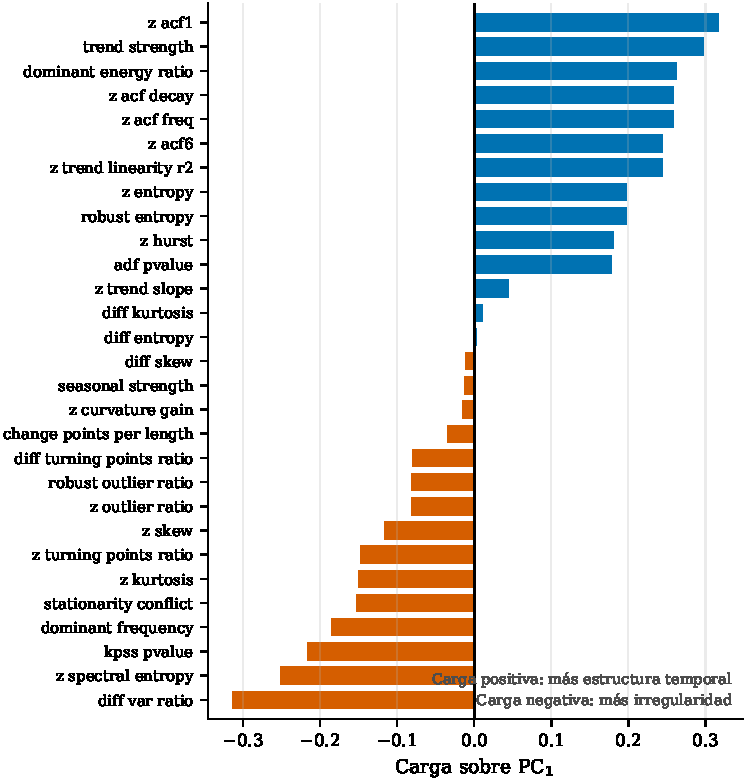
\includegraphics[width=0.62\linewidth]{figuras/fig3_loadings_pc1.pdf}
\caption{Cargas de las 29 características sobre la primera componente principal.
Las cargas positivas corresponden a estructura temporal explotable y las negativas
a irregularidad. La interpretabilidad de estas cargas es lo que distingue al índice
de un escalar de complejidad sin descomposición.}
\label{fig:loadings}
\end{figure}

\paragraph{Cuánta varianza retiene la componente.} $\mathrm{PC}_1$ explica el
26.9\,\% de la varianza del espacio estandarizado de 29 descriptores;
$\mathrm{PC}_2$ el 12.3\,\%, y hacen falta 10 componentes para alcanzar el 80\,\%.
Conviene declararlo porque acota lo que el índice es y lo que no es: \textbf{no es una
representación fiel del espacio de características}, y quien lo use para reconstruir los
descriptores originales obtendrá una aproximación pobre. Es un resumen escalar cuya
validez no descansa en la varianza retenida sino en criterios externos ---la correlación
con el error de pronóstico, la utilidad para decidir fuera de muestra--- que las
secciones siguientes contrastan uno por uno. Que un 27\,\% de varianza baste para las
dos cosas es, de hecho, parte del resultado: la dimensión que separa series fáciles de
difíciles es una sola y no requiere reconstruir el resto del espacio.

\subsection{El índice anticipa el error de pronóstico}\label{sec:anticipa}

Sobre las 99{,}935 series con índice calculado, la correlación con el sMAPE del
pronóstico ingenuo es $r=0.405$ (Pearson) y $\rho=0.399$ (Spearman). Restringiendo
al subconjunto donde las cuatro medidas de complejidad están definidas
($n=96{,}891$), que es la base de comparación justa, $r=0.411$.

La Figura~\ref{fig:indice}(a) muestra que la relación es monótona a lo largo de
todo el rango: el error medio crece de forma sostenida entre deciles del índice, de
$0.059$ a $0.301$. Por cuartiles, los valores son $0.072$, $0.115$, $0.141$ y
$0.236$, un factor de \textbf{3.29} entre extremos.

\begin{figure}[htbp]
\centering
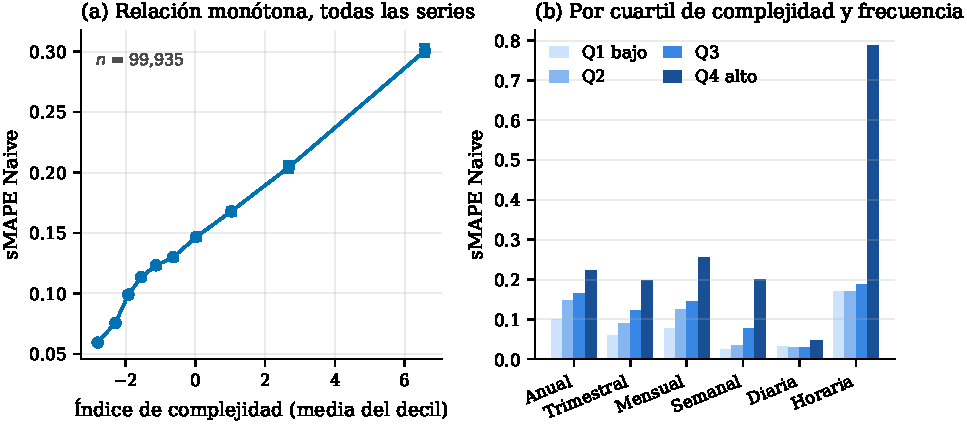
\includegraphics[width=\linewidth]{figuras/fig4_indice_error.pdf}
\caption{(a) Error medio del pronóstico ingenuo por decil del índice, con intervalos
de confianza al 95\,\%. (b) El mismo análisis por cuartil dentro de cada frecuencia.
El gradiente es pronunciado en la frecuencia horaria y practicamente inexistente en
la diaria.}
\label{fig:indice}
\end{figure}

\subsection{El índice no es redundante con las medidas clásicas}\label{sec:redundancia}

El Cuadro~\ref{tab:validacion} compara el índice con las tres medidas establecidas.
El resultado exige una lectura cuidadosa: la complejidad de Lempel-Ziv supera al
índice en correlación de rangos ($\rho=0.429$ frente a $0.399$), mientras que el
índice la supera en correlación lineal ($r=0.411$ frente a $0.362$). Las dos
afirmaciones son ciertas y describen propiedades distintas: LZ ordena las series
algo mejor, el índice modela mejor la magnitud del error.

\begin{table}[htbp]
\centering
\caption{Correlación con el error del pronóstico ingenuo y varianza explicada
($n=96{,}891$). Los $R^{2}$ provienen de regresiones lineales anidadas sobre el
sMAPE del Naive.}
\label{tab:validacion}
\begin{tabular}{lccc}
\toprule
\textbf{Medida} & \textbf{Pearson} & \textbf{Spearman} & \textbf{$R^{2}$} \\
\midrule
Índice de complejidad ($\mathrm{PC}_1$) & \textbf{0.411} & 0.399 & \textbf{0.169} \\
Complejidad de Lempel-Ziv               & 0.362 & \textbf{0.429} & --- \\
\emph{Sample entropy}                   & 0.240 & 0.275 & --- \\
Entropía de permutación                 & 0.054 & 0.062 & --- \\
\midrule
Las tres medidas clásicas en conjunto   & ---   & ---   & 0.132 \\
Índice $+$ medidas clásicas             & ---   & ---   & \textbf{0.183} \\
\bottomrule
\end{tabular}
\end{table}

La regresión resuelve la comparación. El índice, como predictor individual, explica
más varianza del error ($R^{2}=0.169$) que las tres medidas clásicas en conjunto
($R^{2}=0.132$). Conviene ser preciso sobre el alcance de esta afirmación: establece
que el índice supera a \emph{esas tres medidas establecidas}, no que sea superior a
cualquier caracterización de complejidad ni a conjuntos de atributos más ricos. Incorporar las entropías al modelo con el índice mejora el ajuste
un 8\,\%; incorporar el índice al modelo con las entropías lo mejora un 38\,\%. El
aporte incremental es marcadamente asimétrico a favor del índice.

Este resultado es el que sostiene la contribución: un índice construido por
componentes principales sobre descriptores propios podría estar capturando un
artefacto de la representación elegida, y la comparación con medidas independientes
y consolidadas descarta esa posibilidad.

\paragraph{El índice predice también el error del mejor modelo.} Una objeción
razonable es que el índice podría correlacionar con el error del pronóstico ingenuo
por una causa común ---la fuerza de la tendencia, por ejemplo--- sin ser informativo
sobre la dificultad que enfrentan métodos no triviales. Para descartarlo se repite la
correlación contra el \emph{error del oráculo}: el menor sMAPE entre los 27 candidatos
evaluados, serie por serie (Cuadro~S9 del material suplementario).



La correlación con el error del oráculo es igual o superior a la obtenida contra el
error del ingenuo. El índice no está capturando cuán mal se comporta un método
particular, sino \emph{cuán difícil es la serie para cualquier método disponible},
que es la propiedad relevante para una decisión de asignación de modelos.

\subsection{Qué tan estable es el índice}\label{sec:estabilidad}

El índice no se reporta: se usa para decidir. Si una serie cambiara de estrato ante una
perturbación que no cambia su naturaleza, la política enrutaría distinto por razones que
no son de la serie. Se midió entonces sobre 1{,}800 series ---300 por frecuencia---
recalculando los 29 descriptores sobre versiones perturbadas y proyectándolas con el
mismo escalador y la misma componente ajustados sobre los datos originales, que es como
se usaría el índice en la práctica. La cantidad que importa no es la correlación sino la
\textbf{fracción de series que cruza el corte}, porque es el estrato y no el valor lo que
la política consume.

\textbf{Frente al ruido el índice es estable.} Sumando ruido gaussiano de desvío
proporcional al de la serie, cambia de estrato el 1.4\,\% de las series al 1\,\% de ruido
y el 4.8\,\% al 5\,\%, con correlación de Spearman que no baja de $0.988$.

\textbf{Frente al recorte de la historia no lo es.} Recalculando el índice sobre el
último 75\,\% de las observaciones cambia de estrato el 18.9\,\% de las series, y sobre el
último 50\,\% el 32.6\,\%, con Spearman de $0.630$. La primera explicación que cabe ---que
el efecto sea mecánico, porque la longitud es uno de los 29 descriptores--- se descarta:
repitiendo todo con un índice construido sin \texttt{log\_length}, la fracción que cambia
de estrato pasa de 32.6\,\% a 32.3\,\%. \textbf{Son los descriptores de forma los que se
mueven}: con la mitad de la historia, la fuerza de tendencia, la estacional y las
autocorrelaciones describen una serie distinta.

El desglose por frecuencia (Cuadro~S5 del material suplementario) ordena los extremos de
un modo coherente con el resto del trabajo: la horaria es la más estable (Spearman
$0.939$ con media historia) y la diaria la más frágil ($0.278$), el mismo orden que el de
utilidad del índice. Donde hay estructura que medir la medición es reproducible; donde no
la hay, el índice ajusta ruido. \textbf{La consecuencia es una condición de uso y no una
objeción al instrumento}: el índice sirve para estratificar colecciones cuyas series
tienen historia comparable ---el caso de M4 y el de las decisiones que aquí se evalúan---
y la estratificación debe rehacerse cuando la historia disponible cambie de forma
sustancial.


\subsection{La dependencia de la frecuencia}\label{sec:frecuencia}

La capacidad predictiva del índice dista de ser uniforme
(Figura~\ref{fig:frecuencia}). La correlación con el error va de $r=0.736$ en la
frecuencia horaria a $r=0.019$ en la diaria. Reportar únicamente la correlación
agregada sería engañoso: mezcla seis poblaciones con horizontes y dinámicas
distintas, y el valor global puede estar influido por diferencias \emph{entre}
frecuencias más que \emph{dentro} de ellas.

\begin{figure}[htbp]
\centering
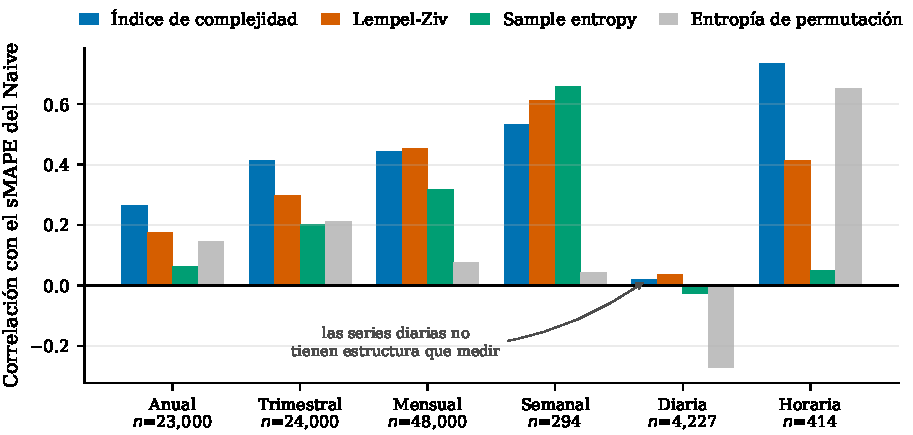
\includegraphics[width=\linewidth]{figuras/fig5_correlacion_frecuencia.pdf}
\caption{Correlación de Pearson con el sMAPE del pronóstico ingenuo, por frecuencia
y por medida de complejidad. Ninguna de las cuatro medidas logra señal apreciable
en la frecuencia diaria.}
\label{fig:frecuencia}
\end{figure}

El caso diario merece atención detenida, porque a primera vista parece una falla
del método. No lo es. Tres evidencias independientes apuntan a que esas series
carecen de estructura explotable:

\begin{enumerate}
\item \textbf{Ninguna medida de complejidad correlaciona} con el error en esa
      frecuencia; la entropía de permutación incluso lo hace en sentido negativo
      ($-0.273$).
\item \textbf{El clustering casi no las separa}: solo 1.7\,\% quedan asignadas al
      grupo complejo, la proporción más baja de las seis frecuencias.
\item \textbf{Ningún modelo supera al benchmark}: ARIMA(1,1,1) obtiene
      $\mathrm{OWA}=1.001$ sobre las series diarias y ninguno de los 27 candidatos
      evaluados baja de $0.979$.
\end{enumerate}

Donde el índice no discrimina, tampoco lo hace ningún método de pronóstico. El
resultado, entonces, es consistente con la hipótesis del trabajo en lugar de
contradecirla.

\paragraph{Corroboración externa del caso diario.} La interpretación anterior
---que la frecuencia diaria carece de estructura explotable y no que el índice falle
en detectarla--- admite una verificación independiente de este trabajo. Los resultados
oficiales de la competencia \cite{m4results} muestran que \emph{los dos métodos
ganadores de M4 pierden contra el benchmark en las series diarias}: el híbrido ES-RNN
de Smyl obtiene allí OWA $=1.046$ y la combinación FFORMA $1.019$, ambos por encima de
$1$. Dos sistemas construidos por equipos especializados y evaluados a ciegas contra
un conjunto de prueba oculto quedan por detrás de un paseo aleatorio desestacionalizado
en una frecuencia entera. La ausencia de señal que el índice reporta en la frecuencia
diaria coincide, por lo tanto, con la ausencia de señal que la competencia misma
documenta.

\subsection{Una partición binaria natural}\label{sec:clusters}

La Figura~S1 del material suplementario presenta las métricas de validación interna. El
coeficiente de Silhouette alcanza su máximo en $k=2$ ($0.334$) y el índice de
Davies-Bouldin su mínimo ($1.531$), ambos con margen amplio sobre cualquier
$k\geq3$. Los criterios de información de los modelos de mezcla gaussiana decrecen
de forma monótona sin codo, lo que no respalda ninguna partición con más grupos.
La coincidencia entre criterios geométricos y de información refuerza la
conclusión.



La partición resultante (Figura~\ref{fig:pca}) separa 79{,}807 series regulares
(79.9\,\%) de 20{,}128 complejas (20.1\,\%). El Cuadro~\ref{tab:clusters} las
caracteriza: el grupo regular presenta autocorrelación de primer rezago de $0.923$
frente a $0.561$, fuerza de tendencia de $0.949$ frente a $0.542$, y un error de
pronóstico ingenuo \textbf{116\,\% mayor} en el grupo complejo.

\begin{figure}[htbp]
\centering
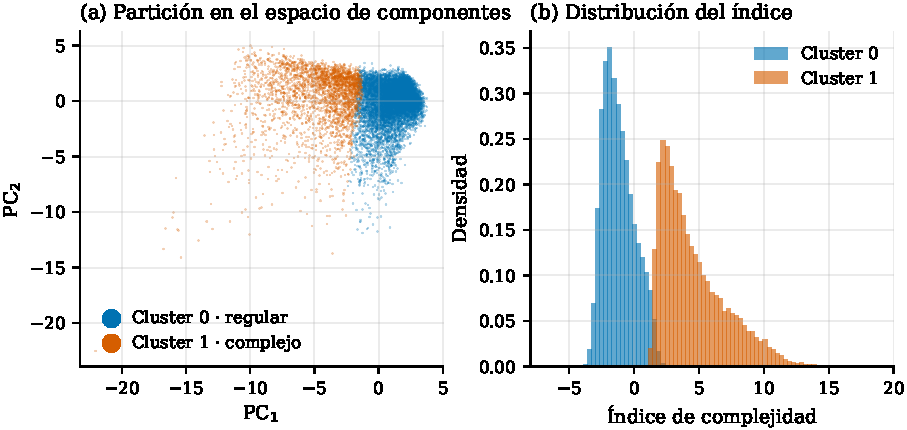
\includegraphics[width=\linewidth]{figuras/fig1_pca_clusters.pdf}
\caption{(a) Proyeccion sobre las dos primeras componentes, con la asignación de
grupos (submuestra de 14{,}000 series para legibilidad). (b) Distribución del
índice de complejidad por grupo: el solapamiento es escaso, lo que indica que la
partición se alinea con el eje que el índice mide.}
\label{fig:pca}
\end{figure}

\begin{table}[htbp]
\centering
\caption{Caracterización de los grupos globales ($k=2$). Los errores de pronóstico
se calculan sobre las 100{,}000 series y las seis frecuencias.}
\label{tab:clusters}
\begin{tabular}{lrr}
\toprule
\textbf{Característica} & \textbf{Grupo 0 (regular)} & \textbf{Grupo 1 (complejo)} \\
\midrule
Series                        & 79{,}807 (79.9\,\%) & 20{,}128 (20.1\,\%) \\
ACF rezago 1                  & 0.923  & 0.561 \\
Fuerza de tendencia STL       & 0.949  & 0.542 \\
Índice de complejidad (media) & $-1.16$ & $+4.60$ \\
sMAPE Naive                   & 0.115  & 0.249 \\
sMAPE ARIMA(1,1,1)            & 0.107  & 0.232 \\
\bottomrule
\end{tabular}
\end{table}

La composición de los grupos varía de forma sistemática entre frecuencias: la
proporción de series asignadas al grupo complejo va de 1.7\,\% en las diarias a
39.1\,\% en las horarias, con las restantes entre 15\,\% y 23\,\%. Sobre la
población mensual completa (48{,}000 series) la partición reproduce el patrón
global (Silhouette $=0.385$, Davies-Bouldin $=1.291$; reparto 79.4\,\% / 20.6\,\%),
sin evidencia de una separación más pronunciada que en el conjunto total.

% =====================================================================
\section{El banco de evaluación}\label{sec:banco}
% =====================================================================

Toda afirmación sobre si una regla de decisión mejora el pronóstico se apoya en
la métrica con la que se la mide. Esta sección construye ese banco: verifica que
la implementación del benchmark reproduce la de la competencia, evalúa el banco
bajo la métrica oficial, y establece qué diferencias entre ellos son reales y
cuáles son ruido. Sin esto, el experimento de la Sección~\ref{sec:decision} no
tendría contra qué contrastarse.

\subsection{Validación del protocolo de evaluación}\label{sec:validacion}

Antes de comparar modelos es necesario verificar que la implementación del
benchmark reproduce la de la competencia; de lo contrario todos los OWA quedan
desplazados. La Figura~S2 del material suplementario y el Cuadro~S2 del material suplementario presentan la
comparación contra los valores publicados \cite{makridakis2020}.





Las tres frecuencias con $m=1$ coinciden de forma exacta, que es lo esperable:
allí Naive2 degenera en el pronóstico ingenuo y no interviene ninguna
descomposición estacional. Las diferencias en las frecuencias estacionales
provienen de que la implementación de descomposición empleada no es idéntica a la
del código original. El desvío global es de $0.016$ puntos de sMAPE.

Como verificación adicional, dos implementaciones independientes del pronóstico
ingenuo ---la del pipeline de modelos y la del módulo de métricas--- producen
valores idénticos (sMAPE $14.280$, MASE $3.305$), al igual que las del ingenuo
estacional ($12.033$, $2.433$).

\subsection{Evaluación del banco bajo OWA}\label{sec:evaluacion}

Se evaluaron \textbf{28 métodos} sobre 5{,}773 series: los tres benchmarks ingenuos de la
competencia ---Naive, Naive estacional y Naive2--- y 25 modelos repartidos en estadísticos
clásicos (ARIMA, SARIMA, ETS, Holt, Holt-Winters, suavizado exponencial), aprendizaje
automático (regresión lineal, LassoLars, bayesiano, SVM, KNN, procesos gaussianos, Random
Forest, Bagging, AdaBoost, XGBoost, LightGBM) e híbridos y neuronales (ARIMA-RF, ARIMA-NN,
SARIMA-NN, perceptrón, ConvNet 1D, LSTM, Transformer, LSTM-Conv1D). Las políticas de las
Secciones~\ref{sec:enrutamiento} y~\ref{sec:combinar}, y el contraste de la
Sección~\ref{sec:friedman}, operan sobre \textbf{27} de esos 28: se excluye Holt-Winters
porque no está definido donde $m=1$ y el diseño exige que cada candidato esté disponible
en toda serie.

Los OWA se reportan reponderados a la población real de M4, porque la muestra
evaluada sobre-representa las frecuencias diaria y horaria (17.3\,\% y 7.2\,\%,
frente a 4.2\,\% y 0.4\,\% en la competencia), que son justamente aquellas donde
varios modelos se descontrolan. La reponderacion se aplica por separado a sMAPE y
MASE antes del cociente, consistente con (\ref{eq:owa}).



Solo seis modelos superan al benchmark (Figura~S5 del material suplementario). ARIMA(1,1,1)
encabeza con $\mathrm{OWA}=0.932$, seguido de SARIMA ($0.934$), LassoLars
($0.973$), regresión lineal ($0.979$), ETS ($0.993$) y Holt-Winters ($0.995$). El
resultado reproduce, en escala reducida, uno de los hallazgos centrales de M4: los
métodos estadísticos clásicos siguen siendo competitivos frente a alternativas de
aprendizaje automático considerablemente más costosas.

\subsection{La inversión en la frecuencia horaria}\label{sec:horaria}

El orden global oculta una inversión completa. La Figura~\ref{fig:heatmap} muestra
el OWA de cada modelo desagregado por frecuencia.

\begin{figure}[htbp]
\centering
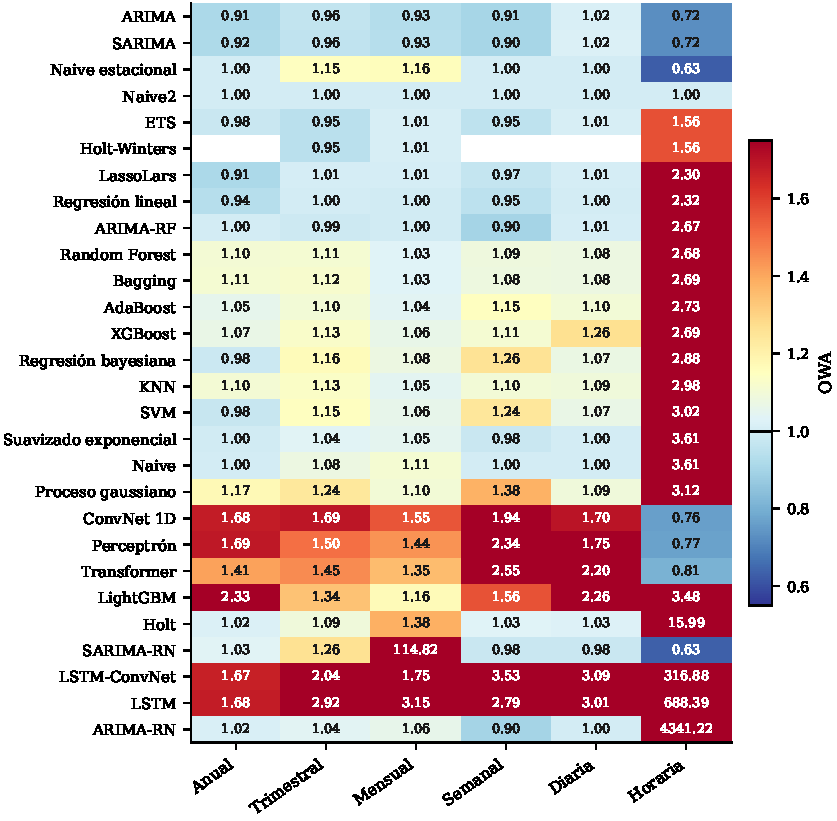
\includegraphics[width=0.72\linewidth]{figuras/fig7_owa_heatmap.pdf}
\caption{OWA por modelo y frecuencia. Los valores mostrados son exactos; la
\emph{escala de color} se satura fuera del rango $[0.55,\,1.75]$ para que las
diferencias relevantes sigan siendo distinguibles pese a los valores extremos de
los modelos que divergen (Cuadro~S3 del material suplementario). La línea negra en la barra
de color marca el benchmark. Las celdas en blanco corresponden a Holt-Winters en
las frecuencias con $m=1$, donde el modelo no aplica. Las redes neuronales pasan
de las peores posiciones a las mejores únicamente en la frecuencia horaria.}
\label{fig:heatmap}
\end{figure}



En la frecuencia horaria el orden se reorganiza por completo. El ingenuo estacional
obtiene el mejor resultado de toda la evaluación ($0.626$), seguido de SARIMA-NN ($0.631$)
y de ARIMA y SARIMA (ambos $0.724$). Las redes neuronales, que en las otras cinco
frecuencias ocupan las últimas posiciones con OWA entre $1.4$ y $1.7$, se ubican aquí por
debajo del benchmark ---ConvNet 1D $0.762$, perceptrón $0.768$, Transformer $0.807$---: el
mismo modelo que resulta 60\,\% peor que Naive2 en el promedio global lo supera en 24\,\%
aquí. La explicación es la disponibilidad de datos, porque con $m=24$, 960 observaciones
por serie y un ciclo diario marcado estas arquitecturas tienen con qué aprender el patrón,
y en el resto de las frecuencias ---mediana de longitud entre 29 y 202 observaciones--- no
lo tienen. Es precisamente el tipo de fenómeno que una selección condicionada por
estructura puede explotar y que una evaluación agregada no dejaría ver.

\subsection{Dos modos de fallo que el promedio esconde}\label{sec:extremos}

Cuatro modelos presentan OWA entre 11 y 365, cifras que a primera vista sugieren un
desempeño inutilizable, pero cuyas medianas se ubican entre $0.9$ y $1.8$. El promedio
está dominado por un puñado de series, y el mecanismo es una asimetría entre las dos
métricas que componen el OWA: \textbf{sMAPE está acotado en 200 y MASE no tiene cota
superior}, de modo que un pronóstico que diverge queda saturado en el primero y arrastra
sin límite el promedio del segundo. El caso testigo es la serie \texttt{H366}, con sMAPE
$=199.99$ y MASE $=127{,}224$.

A ese modo de fallo ---típicamente correcto, catastrófico en pocas series--- se suma uno
distinto, que conviene separar porque tiene otra lectura: LightGBM, el peor del banco,
falla en el \emph{centro} de la distribución y por una propiedad estructural, ya que un
ensamble de árboles predice promedios de hojas y no puede extrapolar fuera del rango
observado. En anual emite un pronóstico plano en el 95.7\,\% de las series.

\textbf{La distinción entre un modelo mal ajustado y uno estructuralmente inadecuado
para una familia de series es exactamente el tipo de heterogeneidad que una regla
condicionada por estructura debería capturar}, y explica por qué LightGBM nunca aparece
en los conjuntos que la Sección~\ref{sec:combinar} selecciona para anual u horaria. La
implicación práctica es que al reportar MASE promedio conviene acompañarlo de la mediana
y del conteo de casos extremos. El desglose completo, con el cuadro por modelo y el
diagnóstico de LightGBM frecuencia por frecuencia, está en la Sección~S2 del material
suplementario.

\subsection{Significancia estadística de las diferencias}\label{sec:friedman}

Las comparaciones anteriores se basan en promedios, que la Sección~\ref{sec:extremos} mostró
frágiles. Para contrastar las diferencias sin esa fragilidad se aplica el
procedimiento estándar de comparación de múltiples métodos sobre múltiples conjuntos de
datos \cite{demsar2006}: se ordenan los modelos \emph{dentro de cada serie}, se contrasta
con Friedman la hipótesis de que todos rinden igual, y se identifican los pares que
difieren con el post-hoc de Nemenyi. Un análisis por rangos es inmune al problema de la
subsección anterior, porque solo importa el orden dentro de cada serie y no cuánto se
aleja el peor pronóstico. El diseño exige que cada modelo se evalúe en cada serie:
Holt-Winters se excluye porque no aplica donde $m=1$ y 26 series se descartan porque algún
ajuste no convergió, de modo que quedan $k=27$ modelos sobre $N=4{,}747$ series.

Friedman rechaza la equivalencia con holgura ($\chi^{2}=13{,}167$, $p<10^{-15}$) y la
diferencia crítica de Nemenyi al 5\,\% es $0.602$ posiciones de rango.

\begin{figure}[htbp]
\centering
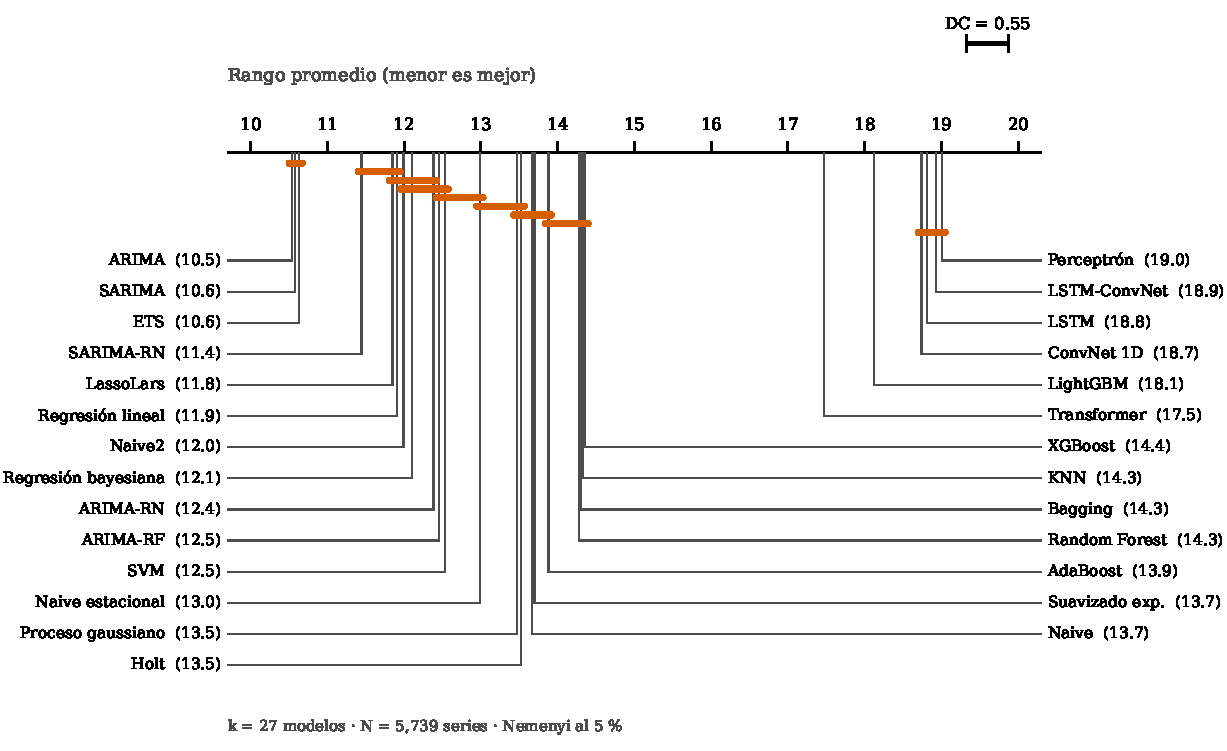
\includegraphics[width=\linewidth]{figuras/fig10_nemenyi.pdf}
\caption{Diagrama de diferencias críticas. Cada modelo se ubica en su rango
promedio sobre las 4{,}747 series; menor es mejor. Las barras horizontales unen
grupos cuyas diferencias no alcanzan la diferencia crítica, es decir, modelos
estadísticamente indistinguibles entre sí.}
\label{fig:nemenyi}
\end{figure}

Tres resultados merecen destacarse.

\paragraph{Hay un empate estadístico en la cima.} ARIMA ($10.55$), SARIMA
($10.58$) y ETS ($10.67$) quedan dentro de la diferencia crítica: sus diferencias
no son significativas. El orden por OWA ---que ubicaba a ETS sexto, detrás de dos
métodos de regresión--- sugería una jerarquía que el test no respalda. La
conclusión defendible no es que ARIMA sea el mejor modelo, sino que \emph{los tres
métodos estadísticos clásicos son equivalentes entre sí y superiores al resto}.

\paragraph{Los modelos que divergen no son malos: son inestables.} SARIMA-RN pasa
del último puesto por OWA ($31.06$) al \textbf{cuarto} por rangos ($11.25$),
indistinguible de ETS. ARIMA-RN pasa del puesto 29 por OWA ($23.45$) al noveno por
rangos ($12.46$). Su comportamiento \emph{típico} es competitivo; lo que los hunde
en el promedio son unas pocas series donde el pronóstico se dispara. Las dos
lecturas son correctas y describen fenómenos distintos: el promedio mide el riesgo
de cola, el rango mide el desempeño habitual. Reportar ambas es lo que permite
distinguir un modelo consistentemente mediocre de uno usualmente bueno pero
ocasionalmente catastrófico ---una distinción que ninguna de las dos métricas
revela por separado.

\paragraph{Las redes neuronales quedan últimas también por rangos.} ConvNet 1D,
perceptrón y LSTM ocupan las posiciones finales con rangos entre $18.5$ y $18.9$,
muy por encima de la diferencia crítica respecto de cualquier método clásico. A
diferencia del caso anterior, aquí el mal desempeño no es un artefacto del
promedio: es sistemático serie por serie.

El análisis se repitió usando MASE en lugar de sMAPE para construir los rangos. Los
dos ordenamientos son prácticamente idénticos (correlación de Spearman $=1.000$;
ningún modelo se desplaza más de una posición), lo que indica que las conclusiones
no dependen de la métrica elegida para ordenar.

% =====================================================================
\section{Qué decisión permite la estructura}\label{sec:decision}
% =====================================================================

Las dos secciones anteriores establecen que el índice \emph{correlaciona} con la
dificultad del pronóstico y que existe un banco de 27 candidatos medido con la métrica
oficial. Ninguna de las dos establece que el índice sea \emph{útil}, que es una
afirmación distinta y más exigente: que usarlo mejore una decisión concreta, evaluada
fuera de muestra. Esta sección la contrasta, y a continuación hace lo que rara vez se
hace con un resultado favorable: mide cuánto falta para el óptimo, verifica si el
faltante se debe al resumen escalar o al enfoque, y termina identificando la causa del
límite.

\subsection{¿Sirve el índice para elegir modelo?}\label{sec:enrutamiento}

Los resultados anteriores establecen que el índice \emph{correlaciona} con la
dificultad del pronóstico. No establecen que \emph{usarlo} mejore una decisión, que
es una afirmación distinta y más exigente. Esta sección la contrasta directamente.

\paragraph{Diseño.} Una regla de enrutamiento es una función que asigna un modelo a
cada serie. El número de estratos de complejidad se fija \textbf{a priori en dos},
justificado por el análisis de conglomerados de la Sección~\ref{sec:clusters}, que identifica $k=2$
mediante criterios internos sin observar ningún error de pronóstico. Esta elección es
por tanto independiente del experimento que sigue: no se selecciona mirando el
desempeño en el conjunto de prueba. El barrido sobre otros valores se reporta más
abajo como análisis de robustez, no como criterio de selección.

Se comparan cuatro reglas:

\begin{description}
\item[A · Fijo] un único modelo para toda la colección, el mejor en entrenamiento.
\item[B · Por frecuencia] el mejor modelo de cada frecuencia.
\item[C · Por índice] el mejor modelo de cada par (frecuencia, estrato de complejidad).
\item[D · Oráculo] el mejor modelo para cada serie individual. No es alcanzable por
      ninguna regla real; se reporta como cota superior.
\end{description}

Cada regla se \textbf{aprende} sobre la mitad de las series y se \textbf{evalúa}
sobre la otra mitad, con partición estratificada por frecuencia y repetida sobre 30
particiones aleatorias. Los cortes de los estratos se calculan únicamente con el
conjunto de entrenamiento y se aplican al de prueba; usar los cuantiles del conjunto
completo introduciría fuga de información. El experimento no reajusta ningún modelo:
reutiliza los errores por serie ya calculados.

\textbf{La política B es el control que da validez al resultado.} La pregunta
relevante no es si enrutar sirve ---evidentemente sí--- sino si el índice aporta algo
por encima de lo que la frecuencia, conocida de antemano y sin costo, ya proporciona.

\begin{table}[htbp]
\centering
\caption{Desempeño de las reglas de enrutamiento sobre el conjunto de prueba.
Promedio y desviación estándar sobre 30 particiones aleatorias, con dos estratos de
complejidad por frecuencia.}
\label{tab:enrutamiento}
\begin{tabular}{llrr}
\toprule
& \textbf{Regla} & \textbf{OWA} & \textbf{Desv.} \\
\midrule
A & Un modelo fijo para toda la colección   & 0.9234 & 0.0083 \\
B & El mejor modelo de cada frecuencia      & 0.9140 & 0.0070 \\
C & \textbf{El mejor de cada frecuencia y estrato} & \textbf{0.8835} & 0.0057 \\
\midrule
D & Oráculo por serie (cota inalcanzable)   & 0.5423 & 0.0038 \\
\bottomrule
\end{tabular}
\end{table}

\paragraph{Resultado.} La política basada en el índice supera a la basada solo en la
frecuencia en \textbf{las 30 particiones}, con una ventaja media de $0.0306$ puntos
de OWA y una prueba de Wilcoxon pareada de $p = 1.9\times10^{-9}$
(Cuadro~\ref{tab:enrutamiento}, Figura~\ref{fig:enrutamiento}a). Expresado sobre la
distancia entre el modelo fijo y el oráculo, la frecuencia por sí sola recorre el
2.4\,\% y la frecuencia junto con el índice recorre el 10.5\,\%: cuatro veces
más.

\begin{figure}[htbp]
\centering
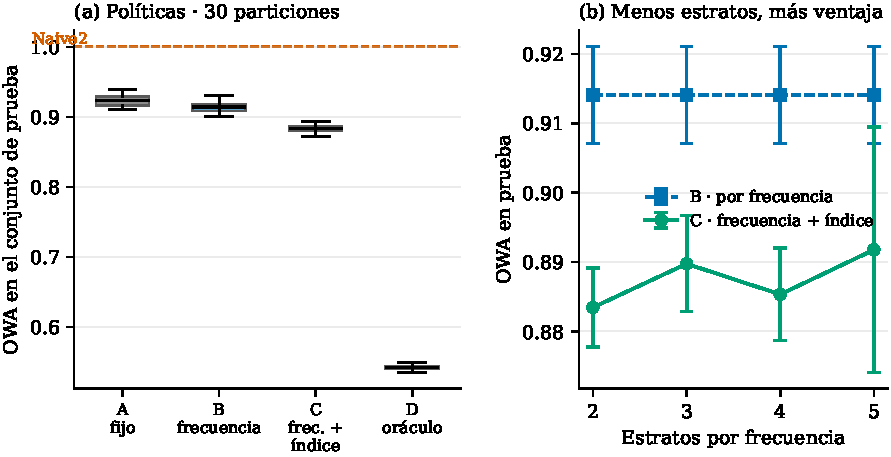
\includegraphics[width=\linewidth]{figuras/fig11_enrutamiento.pdf}
\caption{(a) OWA de cada regla sobre el conjunto de prueba, en 30 particiones
aleatorias. (b) Efecto del número de estratos de complejidad: la ventaja del índice
sobre el enrutamiento por frecuencia es significativa en todos los casos, pero decrece
de forma monótona al aumentar la granularidad.}
\label{fig:enrutamiento}
\end{figure}

\paragraph{Robustez frente al número de estratos.} Repetir el experimento con tres,
cuatro y cinco estratos deja la ventaja sobre el enrutamiento por frecuencia
significativa en los cuatro casos, de modo que el resultado no depende de la
granularidad elegida; la magnitud decrece de forma monótona, lo que es esperable
porque con más estratos cada regla se estima sobre menos series. El valor fijado a
priori ---dos estratos, tomados del análisis de conglomerados--- resulta ser también el
de mejor desempeño fuera de muestra, con una ventaja de $+0.0306$ frente a $+0.0243$,
$+0.0287$ y $+0.0223$ de las demás granularidades. El barrido completo está en el
Cuadro~S4 del material suplementario.


Este resultado admite una lectura que excede al experimento, pero conviene enunciarla con
precisión. El análisis de conglomerados de la Sección~\ref{sec:clusters} identifica $k=2$
mediante criterios internos ---Silhouette, Davies-Bouldin, AIC y BIC--- sin observar ningún
error de pronóstico; el experimento de enrutamiento identifica dos estratos como
granularidad óptima observando únicamente desempeño fuera de muestra. \textbf{Dos
procedimientos independientes coinciden entonces en que la estructura explotable es
binaria}, uno por la geometría del espacio de características y otro por la calidad de las
decisiones que ese espacio habilita.

\textbf{Lo que no debe afirmarse es que sean la misma partición}, y la comprobación
directa lo descarta: el conglomerado reparte las 99{,}935 series en 20{,}128 y 79{,}807,
mientras que el corte por la mediana del índice las reparte en mitades por construcción, y
las dos asignaciones coinciden en el 70.1\,\% de las series frente al 50\,\% que daría el
azar. La relación entre ambas no es de identidad sino de inclusión parcial: el
conglomerado minoritario cae \emph{íntegramente} dentro del estrato de complejidad alta,
sin una sola excepción, de modo que identifica un núcleo del extremo difícil y no su mitad
completa. Lo que ambos procedimientos comparten es la cardinalidad de la partición útil,
no su frontera.

\paragraph{Lo que el índice no captura, y qué mide realmente esa brecha.} La regla
basada en el índice recorre el 10.5\,\% de la distancia hacia el oráculo. Existe, por lo
tanto, información predictiva a nivel de serie individual que un escalar construido por
componentes principales no alcanza a representar.

Conviene ser preciso sobre qué es el 89.5\,\% restante, porque la lectura inmediata
---que esa fracción está disponible y el índice no la aprovecha--- sobrestima lo que
cualquier política podría recuperar. El oráculo elige, serie por serie y mirando la
prueba, el mejor de los 27 candidatos. La distancia que lo separa del modelo fijo mezcla
entonces dos cosas que la métrica no distingue: la información de selección que las
características no capturan, y el error que \emph{ningún} modelo del banco podía evitar
en esa serie. Solo la primera es recuperable, y el experimento no la separa de la
segunda. \textbf{El 89.5\,\% es por lo tanto una cota superior de lo que queda por
ganar, no una medida de señal desaprovechada}, y el mismo reparo vale para las demás
fracciones de hueco que se reportan en este trabajo. Lo que la comparación con el
meta-aprendiz de la Sección~\ref{sec:meta} sí establece, y no depende de esta
ambigüedad, es que la fracción recuperable \emph{por características estructurales}
está prácticamente agotada: veintinueve atributos no llegan mucho más lejos que uno.


\paragraph{Cómo se agrega, y por qué se declara.} Los experimentos de política de esta
sección promedian el error sobre las series de la muestra, mientras que la evaluación de
modelos de la Sección~\ref{sec:evaluacion} pondera cada frecuencia por su participación
en la colección completa. Las dos agregaciones son legítimas y responden a preguntas
distintas ---el desempeño sobre las series efectivamente evaluadas y el desempeño
esperable sobre M4--- pero no son intercambiables: la muestra sobre-representa las
frecuencias diaria y horaria, que pesan el 21\,\% y el 8.7\,\% en ella contra el 4.2\,\%
y el 0.4\,\% en la colección. Para las comparaciones entre políticas de esta sección la
elección no altera ninguna conclusión ---combinar supera a elegir bajo ambas
agregaciones y en cinco de las seis frecuencias por separado--- pero sí lo hace en la
Sección~\ref{sec:nbeats}, donde se reportan las dos de forma explícita.

\subsection{¿Cuánto se pierde frente a un meta-aprendiz completo?}\label{sec:meta}

La regla del apartado anterior usa un escalar y dos estratos. La literatura de
selección de modelos por características ---FFORMS \cite{talagala2018} y FFORMA
\cite{monteromanso2020}--- usa el vector completo de atributos y un meta-modelo
entrenado. La pregunta pertinente no es cuál gana en abstracto, sino \emph{cuánto
cuesta la simplificación}.

\paragraph{Qué se puede y qué no se puede comparar.} FFORMA no es reproducible con
estos datos: combina \emph{pronósticos} con pesos aprendidos, y el registro
disponible guarda el error por serie y modelo, no las predicciones de su conjunto
base, que además proviene de otro pool de métodos. Citar su OWA publicado de 0.838
sobre M4 completo y contrastarlo con 0.884 sobre 5{,}773 series sería engañoso:
distinto conjunto, distinto pool, distinta tarea. Lo que sí es legítimo es
implementar el \emph{enfoque} sobre los mismos datos, el mismo pool y el mismo
protocolo de particiones:

\begin{itemize}
\item[\textbf{E}] \textbf{Clasificador} (estilo FFORMS): un bosque aleatorio sobre
      los 29 atributos predice qué modelo gana en cada serie.
\item[\textbf{F}] \textbf{Regresor por modelo} (estilo FFORMPP): un bosque aleatorio
      por modelo predice su $\log(1+\mathrm{sMAPE})$ y se elige el de menor error
      predicho.
\item[\textbf{E$'$}] \textbf{El mismo clasificador con la pérdida correcta}: se elige el
      modelo que minimiza el arrepentimiento esperado bajo las probabilidades del bosque,
      en lugar de la clase más probable. La agrega el diagnóstico de más abajo.
\end{itemize}

\begin{table}[htbp]
\centering
\caption{El índice frente al meta-aprendizaje sobre el vector completo de 29
atributos. Mismos datos, mismo pool, mismas 30 particiones.}
\label{tab:meta}
\begin{tabular}{llrr}
\toprule
& \textbf{Política} & \textbf{OWA} & \textbf{Cierra} \\
\midrule
A & Modelo fijo global & 0.9234 & --- \\
B & Por frecuencia & 0.9140 & 2.4\,\% \\
C & Frecuencia $\times$ índice (2 estratos) & \textbf{0.8835} & 10.5\,\% \\
E & Clasificador, 29 atributos & 1.4927 & $-152.2$\,\% \\
E$'$ & Clasificador con costos, 29 atributos & \textbf{0.8661} & \textbf{15.0}\,\% \\
F & Regresor por modelo, 29 atributos & 0.8746 & 12.8\,\% \\
D & Oráculo por serie (cota) & 0.5423 & 100\,\% \\
\bottomrule
\end{tabular}
\end{table}

\begin{figure}[htbp]
\centering
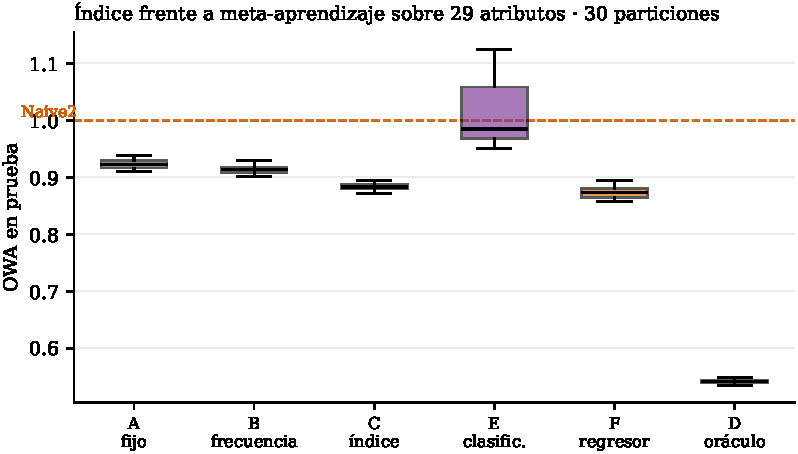
\includegraphics[width=\linewidth]{figuras/fig12_metaaprendizaje.pdf}
\caption{Distribución del OWA de cada política sobre las 30 particiones. La caja del
clasificador (E) se sale del rango del gráfico en varias particiones; su dispersión
---desviación estándar de 2.59 contra 0.006 del índice--- es tan informativa como su
media. E$'$ es el mismo clasificador decidido con la pérdida correcta.}
\label{fig:meta}
\end{figure}

El resultado de la Cuadro~\ref{tab:meta} y la Figura~\ref{fig:meta} tiene dos lecturas
y ninguna es cómoda para una postura extrema.

\paragraph{El aparato completo mejora al índice, y conviene decir cuánto.} La política F
alcanza 0.8746 contra 0.8835 del índice ---ventaja de 0.0089, $p=7.9\times10^{-5}$, con
el índice por delante en 4 de las 30 particiones--- y la mejor de todas es E$'$, con
0.8661. Frente a ella, lo que el aparato completo compra sobre el escalar es 0.0174:
cuatro puntos y medio del recorrido hacia el oráculo. El argumento a favor del índice no
es entonces que lo iguale, sino que recupera siete décimas de lo que consigue con un
escalar y un corte por la mediana, y que el 85\,\% que ninguno de los dos alcanza es el
mismo. La Sección~\ref{sec:dospasos} retoma la comparación con un protocolo que combina
además de elegir, y encuentra una ventaja de $0.0091$ con $k=1$ que se anula con cinco.

\paragraph{El clasificador fracasa, y no por la razón que parece.} La política E queda en
1.4927, peor que no enrutar en absoluto, con una desviación estándar de 2.59 entre
particiones. La lectura inmediata es que la etiqueta ---\emph{cuál} modelo gana en esta
serie--- es ruido, en línea con la Sección~\ref{sec:semillas}. La Sección~S3 del material
suplementario la pone a prueba contra las otras tres explicaciones que caben, sobre las
mismas particiones y el mismo bosque, y obliga a matizarla. El desbalance de clases no es
la causa: corregirlo empeora la partición típica y solo recorta la cola. La etiqueta, en
cambio, sí es casi arbitraria ---en el 11.5\,\% de las series el primero y el segundo
tienen el \emph{mismo} sMAPE--- y acota la exactitud en 18.5\,\%. Pero no es eso lo que
produce el 1.49. Lo produce que la clasificación minimice la pérdida 0--1 mientras el
costo real de equivocarse va de milésimas a órdenes de magnitud: el 1\,\% peor de las
series aporta el 40\,\% del exceso. \textbf{Conservando el mismo bosque y la misma
etiqueta, y cambiando solo la regla de decisión por la que minimiza el arrepentimiento
esperado, el OWA pasa de 1.4927 a 0.8661} ---la política E$'$---, mejor que el índice en
las 30 particiones y que el regresor en 22 de 30. La advertencia para quien implemente
selección por características sobrevive con otra razón: predecir el ganador y creerle es
frágil, pero no porque la etiqueta sea ruido ---el regresor usa la misma--- sino porque
esa formulación descarta la estructura de costos.


\subsection{¿El límite es de la caracterización o de elegir?}\label{sec:combinar}

Los dos apartados anteriores comparten un supuesto que no se hizo explícito: que la
caracterización sirve para \emph{elegir} un modelo. Las políticas B, C, E y F asignan a
cada serie un método y descartan el resto. Hay una razón concreta para dudar de que ese
sea el uso correcto de la caracterización: FFORMA \cite{monteromanso2020} obtuvo el
segundo lugar en M4 con OWA $=0.838$ usando también atributos de series, pero
\emph{combinando} los pronósticos de nueve métodos con pesos aprendidos, sin elegir
ninguno. Si el techo medido fuera del enfoque, ese resultado no debería existir.

\paragraph{Diseño.} Se agregan al mismo protocolo dos familias de políticas que
combinan en lugar de elegir. Para cada partición y cada estrato, se ordenan los modelos
por OWA \emph{en entrenamiento} y se promedian los $k$ mejores sobre las series de
prueba; el promedio simple es deliberado, porque es la forma de combinación más austera
que existe y la que la propia competencia usa como benchmark. La familia $B_k$ combina
dentro de cada frecuencia y la familia $G_k$ dentro de cada frecuencia $\times$ estrato
de complejidad. Con $k=1$ ambas se reducen a las políticas B y C ya vistas, de modo que
la comparación es continua.

\begin{table}[htbp]
\centering
\caption{Elegir un modelo frente a combinar $k$. La columna de aporte es la diferencia
entre combinar por frecuencia y combinar por frecuencia $\times$ estrato: mide lo que
agrega el índice a igual número de modelos combinados.}
\label{tab:combinar}
\begin{tabular}{crrrcr}
\toprule
$k$ & \textbf{$B_k$} & \textbf{$G_k$} & \textbf{Aporte} &
\textbf{$G$ mejor} & \textbf{$p$} \\
  & \textbf{frecuencia} & \textbf{frec.$\times$índice} & \textbf{del índice} & & \\
\midrule
1 & 0.9187 & 0.8869 & $+0.0318$ & 30/30 & $1.9\times10^{-9}$ \\
2 & 0.8951 & 0.8787 & $+0.0165$ & 20/30 & $6.1\times10^{-4}$ \\
3 & 0.8761 & 0.8688 & $+0.0073$ & 26/30 & $3.9\times10^{-7}$ \\
4 & 0.8745 & 0.8672 & $+0.0073$ & 27/30 & $2.0\times10^{-7}$ \\
5 & \textbf{0.8725} & \textbf{0.8647} & $+0.0078$ & 25/30 & $4.4\times10^{-6}$ \\
\midrule
\multicolumn{2}{l}{Oráculo por serie (cota)} & 0.5448 & & & \\
\bottomrule
\end{tabular}
\end{table}

\paragraph{Por qué $B_1$ no coincide con la política B de la
Sección~\ref{sec:enrutamiento}.} Ambas eligen el mejor modelo de cada frecuencia sobre las
mismas 5{,}674 series y el mismo banco, con métricas que coinciden dígito a dígito, pero
$B_1$ da $0.9187$ y B daba $0.9140$. La diferencia es de \emph{partición}: allá cada
frecuencia se divide en mitades exactas y aquí cada serie se asigna por sorteo
independiente, de modo que el tamaño de entrenamiento fluctúa. Repitiendo B bajo los dos
esquemas sobre los mismos datos se obtiene $0.9141$ y $0.9181$, lo que reproduce la
brecha. \textbf{Las cifras son comparables dentro de cada experimento y no entre ellos.}

El Cuadro~\ref{tab:combinar} y la Figura~\ref{fig:combinar} contienen tres resultados.

\paragraph{Las dos decisiones pesan lo mismo, y conviene no afirmar más que eso.} Pasar
de elegir un modelo a promediar cinco mejora el OWA en $0.0462$ dentro de la política por
frecuencia y en $0.0222$ dentro de la política por índice. El aporte del índice sobre la
frecuencia, que la Sección~\ref{sec:enrutamiento} presentaba como el resultado central,
es de $0.0318$. Las dos cantidades son del mismo orden, y la tentación de declarar
ganadora a una de ellas no resiste el error de muestreo: un bootstrap que remuestrea
series dentro de cada frecuencia y promedia sobre particiones sitúa la ganancia de
combinar en $+0.0267$ (IC 95\,\% $[+0.0143,\ +0.0393]$) y la de estratificar en
$+0.0214$ ($[+0.0110,\ +0.0328]$). \textbf{Ambas son significativas por separado; su
diferencia, $+0.0053$ con intervalo $[-0.0148,\ +0.0254]$, no lo es.} Lo que la evidencia
sostiene es que son dos decisiones de magnitud comparable, y que la literatura de
pronóstico por características atiende solo a una de ellas.

\paragraph{El aporte del índice decae al combinar, hasta dejar de ser detectable.}
$G_k$ supera a $B_k$ para todo $k$ evaluado, pero la magnitud decrece de forma monótona y
la evidencia que la sostiene se agota antes que la serie de puntos estimados. Con un
remuestreo de \emph{series} ---la unidad que corresponde, según se argumenta más abajo---
el aporte es $+0.0215$ con intervalo $[+0.0110,\ +0.0326]$ al elegir un modelo y
$+0.0131$ con $[+0.0022,\ +0.0233]$ al combinar dos, ambos claramente por encima de cero.
A partir de ahí los intervalos lo contienen: $+0.0055$ con $[-0.0024,\ +0.0139]$ para
$k=3$, $+0.0018$ con $[-0.0056,\ +0.0098]$ para $k=4$ y $+0.0042$ con
$[-0.0043,\ +0.0120]$ para $k=5$.

\textbf{La lectura defendible es que la combinación absorbe aquello que la
estratificación resolvía, hasta un punto en que el aporte del índice ya no se distingue
de cero.} Está establecido donde la política \emph{elige}, y no lo está en los tamaños de
conjunto que esta sección encuentra mejores. Decir que la caracterización se \emph{reubica}
hacia decidir qué conjunto combinar iría más allá de lo que estos datos permiten: lo que
muestran es que su utilidad es máxima al seleccionar y se diluye al combinar.

\paragraph{Y el techo sigue siendo bajo.} La mejor política evaluada, $G_5$, alcanza
$0.8647$ y recorre el 14.4\,\% de la distancia entre el control por frecuencia y el
oráculo por serie, frente al 8.5\,\% de la política que elige. El aporte crece, y aun
así el grueso de esa distancia ---con el reparo sobre su interpretación que introduce la
Sección~\ref{sec:enrutamiento}--- queda sin recorrer. La conclusión de la
Sección~\ref{sec:meta} se mantiene con una corrección importante: el límite no proviene
de haber resumido la estructura en un escalar \emph{ni} de haber elegido en lugar de
combinar, porque corregir lo segundo apenas duplica un aporte que sigue siendo pequeño.

\begin{figure}[htbp]
\centering
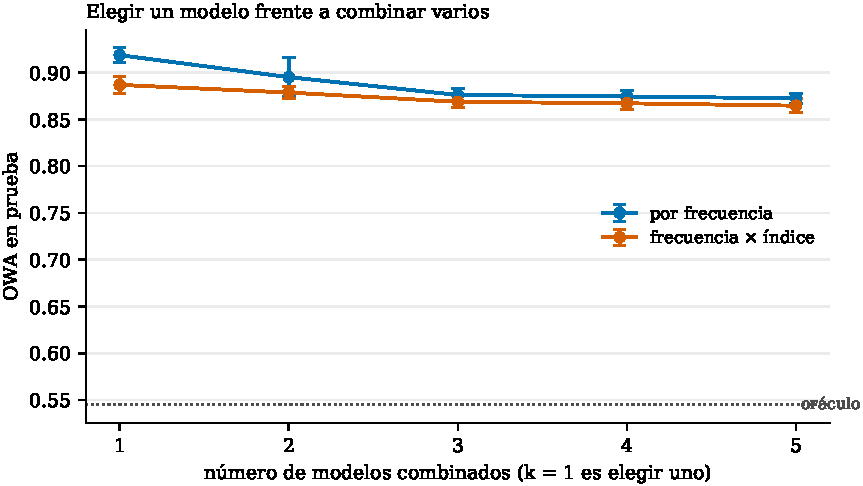
\includegraphics[width=0.82\linewidth]{figuras/fig13_combinar.pdf}
\caption{OWA en prueba según cuántos modelos se combinan, con desviación estándar sobre
las 30 particiones. En $k=1$ ambas curvas son las políticas B y C. La separación entre
curvas es el aporte del índice; la pendiente de cada curva es el aporte de combinar.}
\label{fig:combinar}
\end{figure}

\paragraph{Control: promediar no alcanza, hay que saber qué promediar.} La objeción
inmediata a lo anterior es que el mérito sea del promedio y no de la información que
decide qué promediar. El Cuadro~\ref{tab:controles} la contesta. Promediar cinco modelos
sorteados al azar del banco produce OWA $=5.60$, un desastre previsible porque el banco
contiene modelos que divergen. El control exigente es el segundo: sortear cinco
\emph{dentro de los diez mejores de entrenamiento} ---eliminando así la explicación
fácil--- todavía deja OWA $=1.26$ frente a $0.870$ de los cinco mejores. Saber el orden
fino vale $0.39$ puntos de OWA, en las 30 particiones.
\textbf{La combinación no sustituye a la caracterización: la necesita.}

\begin{table}[htbp]
\centering
\caption{Controles sobre la política de combinación. El primero pregunta si basta
promediar; el segundo, si $k=5$ está ajustado a la prueba.}
\label{tab:controles}
\begin{tabular}{lr}
\toprule
\textbf{Política} & \textbf{OWA} \\
\midrule
\multicolumn{2}{l}{\emph{¿Basta con promediar?}} \\
\quad 5 modelos al azar del banco completo & 5.60 \\
\quad 5 al azar dentro de los 10 mejores en entrenamiento & 1.26 \\
\quad \textbf{los 5 mejores en entrenamiento} & \textbf{0.870} \\
\midrule
\multicolumn{2}{l}{\emph{¿Está $k=5$ ajustado a la prueba?}} \\
\quad $k$ fijado en 5 & 0.870 \\
\quad \textbf{$k$ elegido en entrenamiento, por frecuencia} & \textbf{0.868} \\
\bottomrule
\end{tabular}
\end{table}

\paragraph{El número de modelos no está ajustado a la prueba.} Fijar $k=5$ porque es el
mejor valor observado sobre el conjunto de prueba sería el mismo atajo que este trabajo
descarta en otros puntos. Se implementó por lo tanto una política que elige $k$
\emph{dentro de la mitad de entrenamiento} y por frecuencia, y su desempeño es
\emph{mejor} que el de $k$ fijo ($0.868$ contra $0.870$), de modo que la elección no
introduce sobreajuste sino que lo evita. Los valores que selecciona son interpretables:
cinco en anual y mensual, cuatro en trimestral y horaria, dos en semanal y
\textbf{uno en diaria}. Que la frecuencia sin estructura explotable
(Sección~\ref{sec:frecuencia}) sea también la única donde la regla decide no combinar es
un chequeo de coherencia que no se buscó.

\paragraph{El conjunto que se combina es inestable, y eso confirma el mecanismo.} Una
objeción posible es que la comparación favorezca a la combinación si el conjunto de los
cinco mejores varía entre particiones. Conviene separar dos cosas. La comparación es
simétrica en información: ambas políticas observan \emph{solo} la mitad de
entrenamiento, y la diferencia está en cuántos modelos llevan de ahí a la prueba, no en
qué saben. Pero la inestabilidad existe y merece reportarse: la similitud de Jaccard
media del conjunto de cinco entre particiones va de $0.34$ en diaria a $0.71$ en
horaria, con valores en torno a $0.45$ en el resto; es decir, cerca de la mitad de los
integrantes cambia de una partición a otra. Lejos de debilitar el resultado, esa
inestabilidad \emph{es} el mecanismo: si el ordenamiento de modelos fuera estable,
quedarse con el primero sería una decisión segura. No lo es, y por eso promediar cinco
resulta más robusto que apostar a uno. Es la misma inestabilidad que la
Sección~\ref{sec:semillas} mide directamente, y la razón por la que el clasificador de la
Sección~\ref{sec:meta} no logra identificar al ganador ---aunque, según se vio allí, no
sea lo que hunde su OWA---.

\paragraph{Sobre qué se remuestrea, y por qué cambia la conclusión.} Las 30 particiones
no son 30 muestras independientes: son re-divisiones de las mismas 5{,}674 series. Un
contraste que las trate como réplicas ---una prueba de Wilcoxon sobre particiones, o un
\emph{bootstrap} que remuestree esas 30 diferencias--- responde si el aporte es
\emph{consistente} al volver a dividir esta muestra, que es una afirmación de
reproducibilidad interna y es válida como tal. No responde si el aporte sobreviviría a
haber sorteado otras series, que es lo que hace falta para generalizar, y por eso produce
intervalos demasiado angostos.

Remuestreando series dentro de cada frecuencia y promediando sobre particiones dentro de
cada réplica, los intervalos resultan \textbf{entre tres y seis veces más anchos} que los
que se obtienen remuestreando particiones, y tres de los cinco pasan a contener el cero.
Las cifras del párrafo anterior son las de este procedimiento. El contraste por
particiones se conserva donde corresponde ---para afirmar consistencia, no
significancia--- y se declara como tal.

\paragraph{Coherencia con FFORMA.} El resultado reconcilia el techo medido con el
segundo puesto de FFORMA en lugar de contradecirlo. Promediar cinco modelos con pesos
iguales dentro de dos estratos alcanza $0.8647$; FFORMA combina nueve con pesos
aprendidos y alcanza $0.838$ sobre la colección completa. Los dos valores pertenecen al
mismo régimen, y la diferencia entre ellos es atribuible a la sofisticación de los pesos
y del pool, no a un cambio de enfoque. Lo que la evidencia de este trabajo descarta no
es el uso de características de series, sino su uso \emph{para seleccionar}, que es
precisamente lo que FFORMA no hace y lo que la variante como clasificador
(Sección~\ref{sec:meta}) lleva al extremo.

\paragraph{¿Depende algo de estos 29 descriptores en particular?} El conjunto se
eligió por interpretabilidad y cobertura de familias, no por un procedimiento de
selección, y cabe preguntar cuánto de lo anterior depende de esa elección. La referencia
canónica es catch22 \cite{lubba2019}, 22 características filtradas de las 4{,}791 de
hctsa por desempeño de clasificación y redundancia mutua. Se construyó un índice análogo
---negativo de la primera componente principal sobre las 22 características
estandarizadas, con el signo fijado únicamente con la mitad de entrenamiento--- y se lo
sometió a las mismas pruebas.

\begin{table}[htbp]
\centering
\caption{El índice propio frente a uno construido sobre catch22, bajo el mismo protocolo
de 30 particiones. Valores de OWA; menor es mejor.}
\label{tab:catch22}
\begin{tabular}{crrrr}
\toprule
$k$ & \textbf{Índice propio} & \textbf{catch22} & \textbf{Diferencia} & \textbf{$p$} \\
\midrule
1 & 0.8802 & 0.8793 & $-0.0008$ & $0.25$ \\
2 & 0.8744 & \textbf{0.8710} & $-0.0034$ & $7.1\times10^{-5}$ \\
3 & 0.8637 & \textbf{0.8614} & $-0.0023$ & $3.2\times10^{-3}$ \\
4 & 0.8607 & 0.8602 & $-0.0005$ & $0.31$ \\
5 & 0.8592 & \textbf{0.8543} & $-0.0049$ & $8.9\times10^{-5}$ \\
\bottomrule
\end{tabular}
\end{table}

\textbf{El conjunto canónico rinde al menos tan bien como el propio.} catch22 empata en
$k=1$ y $k=4$ y supera al índice propio en los otros tres, siempre por márgenes que no
pasan de $0.005$ de OWA. El sentido del resultado no cambia por eso, y si acaso se
refuerza: un conjunto de características construido por un criterio opuesto ---filtrado
automático por desempeño de clasificación sobre 93 colecciones, y no elegido por
interpretabilidad--- no abre ningún margen que el índice propio estuviera desaprovechando. En correlación con el error del
pronóstico ingenuo el reparto también es parejo ---catch22 es mejor en mensual, semanal y
diaria; el índice propio en trimestral, horaria y anual. La conclusión conviene enunciarla
sin adornos: los 29 descriptores no son la fuente del resultado, y tampoco lo serían 22
seleccionados por un procedimiento distinto. Lejos de debilitar el trabajo, esto refuerza
su tesis: si dos caracterizaciones construidas con criterios opuestos rinden igual, es
porque el margen disponible para la caracterización es estrecho, y lo que decide está en
otra parte.

\subsection{Frente a un meta-aprendiz publicado}\label{sec:dospasos}

La Sección~\ref{sec:meta} comparó el índice contra dos formulaciones propias de
meta-aprendizaje, pero no contra un método publicado. El más pertinente es el
esquema de dos pasos de Vaiciukynas y colaboradores \cite{vaiciukynas2021}, que
sobre datos de M4 entrena un meta-aprendiz para \emph{ordenar} los métodos y un
segundo para predecir el \emph{tamaño} del ensamble de cada serie. Es exactamente
la generalización por serie de la regla de la Sección~\ref{sec:combinar}, que ordena
y fija el tamaño por estrato.

\paragraph{Por qué no basta con citar su cifra.} El trabajo reporta sMAPE $=9.21$
sobre M4, pero evaluado en 12{,}561 series microeconómicas y no en las 100{,}000: su
Theta de referencia da $11.05$ cuando el Theta oficial de la competencia da $12.309$.
Son escalas distintas, y ponerlas en la misma tabla induciría al error igual que con
FFORMA. Lo que sí informa es implementar el enfoque sobre estos datos, este pool y este
protocolo. El paso 1 entrena un bosque aleatorio por modelo que predice su
$\log(1+\mathrm{sMAPE})$ a partir de los 29 atributos, agrupando las seis frecuencias, y
ordena los modelos de cada serie por error predicho; el paso 2 entrena otro bosque que
predice el $k$ óptimo de cada serie.

\begin{table}[htbp]
\centering
\caption{El índice de dos estratos frente al ordenamiento por serie con los 29
atributos, a igual número de modelos combinados. Treinta particiones.}
\label{tab:dospasos}
\begin{tabular}{crrrr}
\toprule
$k$ & \textbf{Índice} & \textbf{Meta-aprendiz} & \textbf{Diferencia} & \textbf{$p$} \\
  & \textbf{2 estratos} & \textbf{29 atributos} & & \\
\midrule
1 & 0.8823 & 0.8855 & $+0.0032$ & $0.84$ \\
2 & 0.8769 & \textbf{0.8682} & $-0.0086$ & $0.014$ \\
3 & 0.8683 & \textbf{0.8613} & $-0.0070$ & $0.015$ \\
4 & 0.8665 & 0.8614 & $-0.0052$ & $0.097$ \\
5 & 0.8625 & 0.8655 & $+0.0030$ & $0.18$ \\
\midrule
\multicolumn{5}{l}{\emph{Dos pasos completo, con $k$ aprendido por serie:}
  0.8647 \quad ($p=0.84$)} \\
\bottomrule
\end{tabular}
\end{table}

\paragraph{El resultado precisa el de la Sección~\ref{sec:meta}.} Ordenar por serie con
los 29 atributos \emph{sí} supera al escalar de dos estratos en la zona intermedia, con
ventaja significativa en $k=2$ y $k=3$. Pero no la tiene en los extremos: con $k=1$,
$k=4$ y $k=5$ las dos reglas son indistinguibles. El esquema de dos pasos completo
alcanza $0.8647$ contra $0.8625$ del índice, diferencia sin significancia ($p=0.84$), y
lo hace con el triple de dispersión entre particiones ($0.0161$ contra $0.0057$). El tamaño de ensamble que aprende a predecir ronda entre
$2.1$ en diaria y $2.7$ en horaria.

De ahí la formulación precisa del aporte de este trabajo, que corrige por matiz la de
la Sección~\ref{sec:meta}: \textbf{cuanto más se combina, menos importa qué tan
sofisticada sea la caracterización}. Con $k=1$ el aparato completo ---veintinueve
atributos y veintisiete regresores por partición--- compra $0.0091$ de OWA sobre un
escalar y un corte por la mediana; con $k\ge4$ no compra nada medible. El índice no es
mejor que un meta-aprendiz: llega al mismo lugar con una fracción del aparato, y sólo
una vez que se combina.

\subsection{¿Sobrevive con un banco moderno?}\label{sec:nbeats}

Todo lo anterior se apoya en un banco de 27 candidatos cuyas arquitecturas neuronales son
genéricas y se ajustan serie por serie. La objeción es directa y hay que contestarla con
datos: si el banco incluyera un modelo global moderno, ¿se sostendrían las conclusiones
sobre políticas? Para responderla se entrenó N-BEATS \cite{oreshkin2020} sobre las mismas
series, en su versión genérica ---pilas de bloques densos con conexión residual doble,
donde el \emph{backcast} de cada bloque se resta de la entrada del siguiente--- con una
red por frecuencia entrenada sobre \emph{todas} las series de esa frecuencia y pérdida
sMAPE directa.

\textbf{El estatuto de esta sección conviene fijarlo antes de leer sus números.} Los 27
modelos del banco se ajustan serie por serie sobre la muestra evaluada; N-BEATS se
entrena sobre las 23{,}000 series anuales o las 48{,}000 mensuales completas. La
comparación no enfrenta entonces dos arquitecturas en igualdad de condiciones, sino dos
regímenes de acceso a datos, y parte de cualquier margen que aparezca mide ese acceso y
no el modelo. Por eso \textbf{el análisis principal de este trabajo es el del banco
clásico, donde todos los candidatos se ajustan igual}, y esta sección funciona como
contraste declarado: su pregunta no es cuál modelo gana, sino si la conclusión sobre
\emph{políticas} ---elegir contra combinar--- resiste la aparición de un componente
dominante en el banco. Para esa pregunta la asimetría no estorba, porque las dos
políticas operan sobre el mismo banco sea cual sea su composición.

\paragraph{Cinco semillas, no una.} Reportar una red a partir de una sola corrida sería
incoherente con la Sección~\ref{sec:semillas}, así que se entrenaron cinco semillas por
frecuencia. La precaución resultó necesaria: el Cuadro~\ref{tab:nbeats} muestra que en
la frecuencia semanal el rango entre semillas es de $2.69$ puntos de OWA, de modo que
una corrida aislada habría permitido afirmar cualquier cosa. La corrida individual que
se obtuvo primero daba $0.7250$ en semanal ---mejor que todo el banco--- y la media
sobre cinco semillas es $1.28$.

\begin{table}[htbp]
\centering
\caption{N-BEATS sobre cinco semillas. La última columna indica si se puede afirmar que
supera al mejor de los 27 candidatos: sólo cuando \emph{todas} las semillas quedan del
mismo lado.}
\label{tab:nbeats}
\begin{tabular}{lrrrrl}
\toprule
\textbf{Frecuencia} & \textbf{Media} & \textbf{Desvío} & \textbf{Rango} &
\textbf{Mejor de los 27} & \textbf{¿Lo supera?} \\
\midrule
Anual      & 0.8223 & 0.0038 & 0.011 & 0.9139 & sí, en todas \\
Trimestral & 0.9083 & 0.0077 & 0.023 & 0.9456 & sí, en todas \\
Horaria    & 0.4178 & 0.0055 & 0.015 & 0.6260 & sí, en todas \\
Diaria     & 0.9832 & 0.0046 & 0.012 & 0.9791 & depende de la semilla \\
Semanal    & 1.2828 & 1.0636 & \textbf{2.692} & 0.8971 & depende de la semilla \\
Mensual    & 5.2442 & 3.2344 & \textbf{8.930} & 0.9325 & no, en ninguna \\
\bottomrule
\end{tabular}
\end{table}

\paragraph{La mediana entre semillas es el remedio, y el promedio no.} Agregar las cinco
corridas por mediana lleva la frecuencia semanal a $0.7136$ ---mejor que todo el
banco--- mientras que el promedio la deja en $1.1696$. La diferencia es que la mediana
descarta la corrida divergente y el promedio la incorpora. Es, sobre estos datos, la
misma conclusión que la literatura de combinación establece para la agregación robusta
\cite{wang2023}, y la razón por la que el modelo entra al banco como mediana de cinco
semillas y no como una corrida.

\paragraph{La frecuencia mensual no converge.} Con esta implementación, N-BEATS falla de
forma sistemática en mensual: sMAPE mediano $31.3$ frente a $14.4$ del benchmark, en las
cinco semillas, y no por unas pocas series divergentes sino en el centro de la
distribución. El fallo se documenta como limitación y no se disimula; su efecto sobre lo
que sigue es que la política óptima debe seguir eligiendo otro modelo en esa frecuencia,
cuando con una implementación correcta probablemente no haría falta.

\paragraph{Dónde se invierte la conclusión, y dónde no.} N-BEATS domina cuatro de las
seis frecuencias por márgenes grandes: $+0.231$ sobre el segundo en horaria, $+0.184$ en
semanal, $+0.099$ en anual y $+0.060$ en trimestral. Repetido el experimento de la
Sección~\ref{sec:combinar} sobre el banco ampliado, el resultado cambia \emph{en esas
frecuencias} pero no necesariamente en el agregado, y la distinción importa
(Cuadro~\ref{tab:inversion}).

\begin{table}[htbp]
\centering
\caption{Elegir el mejor modelo frente a combinar los cinco mejores, por frecuencia, con
N-BEATS en el banco. La inversión ocurre donde hay un modelo dominante; en mensual, donde
N-BEATS no converge, combinar sigue ganando.}
\label{tab:inversion}
\begin{tabular}{lrrrl}
\toprule
\textbf{Frecuencia} & \textbf{Peso en M4} & \textbf{Elegir uno} &
\textbf{Combinar cinco} & \textbf{Gana} \\
\midrule
Anual      & 23.0\,\% & \textbf{0.8136} & 0.8350 & elegir \\
Trimestral & 24.0\,\% & 0.8901 & 0.8900 & empate \\
Mensual    & 48.0\,\% & 0.9315 & \textbf{0.9040} & combinar \\
Semanal    &  0.4\,\% & \textbf{0.7136} & 0.7970 & elegir \\
Diaria     &  4.2\,\% & \textbf{0.9791} & 0.9901 & elegir \\
Horaria    &  0.4\,\% & \textbf{0.3947} & 0.5389 & elegir \\
\midrule
\multicolumn{2}{l}{Agregado, pesos poblacionales de M4} & 0.8935 & \textbf{0.8865} & combinar \\
\multicolumn{2}{l}{Agregado, promedio sobre la muestra} & \textbf{0.8452} & 0.8649 & elegir \\
\bottomrule
\end{tabular}
\end{table}

Elegir supera a combinar en las cuatro frecuencias donde N-BEATS domina, empata en
trimestral, y pierde en mensual, que es justamente donde el modelo no converge. El
agregado depende entonces de cómo se pondere: con los pesos poblacionales de M4 ---donde
mensual concentra el 48\,\%--- el orden nominal favorece a combinar por $0.007$;
promediando sobre la muestra evaluada ---que sobre-representa diaria y horaria---
favorece a elegir por $0.020$. \textbf{Ninguna de las dos diferencias resiste el error de
muestreo}, y conviene decirlo antes que elegir la ponderación que convenga. Un bootstrap
de 600 réplicas remuestrea series dentro de cada frecuencia y rehace el protocolo
completo, promediando sobre las mismas 30 particiones que produce el número reportado.
La diferencia agregada con pesos poblacionales queda en $+0.0021$, con intervalo de
confianza del 95\,\% $[-0.0100,\ +0.0132]$, que contiene el cero; combinar resulta mejor
en el 34\,\% de las réplicas. El mismo bootstrap sobre el banco clásico da $-0.0441$ con
intervalo $[-0.0577,\ -0.0307]$ y combinar gana en el 100\,\% de las réplicas, de modo
que el resultado de la Sección~\ref{sec:combinar} no depende de la muestra y este sí.

\textbf{La afirmación defendible no es que la conclusión se invierta en el agregado
---en el agregado las dos políticas empatan--- sino que se invierte en cada frecuencia
donde existe un modelo dominante}, y que su aparición en el agregado dependerá de qué
fracción de la colección tenga uno. Aquí son cuatro de seis frecuencias, pero apenas el
28\,\% de las series.

Conviene precisar qué clase de indeterminación es esta, porque la lectura natural
---que falta muestra en mensual, la frecuencia que aporta el 48\,\% del peso
poblacional y la única de las tres grandes donde N-BEATS no converge--- no resiste la
comprobación. Repitiendo el bootstrap con el error de muestreo mensual anulado, que es
el límite de evaluar sus 48{,}000 series en lugar de 1{,}000, el intervalo queda en
$[-0.0052,\ +0.0118]$ y sigue conteniendo el cero. El remuestreo de la frecuencia
mensual explica apenas el 13\,\% de la varianza de la diferencia; el resto se reparte
entre anual, trimestral y diaria, cuyas muestras son igual de pequeñas frente a sus
poblaciones. \textbf{Ningún volumen de cómputo adicional en mensual cierra este
intervalo}, y el motivo es que no hay nada que cerrar: la diferencia real está acotada
por debajo de $0.014$ OWA en cualquier dirección. Con este banco las dos políticas
empatan dentro de un margen estrecho, que es una conclusión y no una carencia. La
diferencia entre esto y la Sección~\ref{sec:combinar} ---donde combinar gana por
$0.042$ y el intervalo entero queda de un solo lado del cero--- es justamente el punto del
artículo: lo que decide es la dispersión del banco, y un banco con un modelo dominante
la comprime hasta volver indistinguibles las dos políticas.

\paragraph{Dos verificaciones sobre el papel de la frecuencia mensual.} Que el único
contrapeso sea la frecuencia donde la implementación falla exige comprobar que la
conclusión no sea un subproducto de ese fallo. La primera verificación no usa ningún dato
sintético: restringidas las políticas a las \emph{cinco frecuencias donde N-BEATS sí
converge} ---el 52\,\% de la colección--- elegir supera a combinar por $0.0159$ de OWA,
en 29 de 30 particiones ($p=5.6\times10^{-9}$). La inversión, donde el modelo funciona,
es sólida.

La segunda pregunta cuánta calidad haría falta en mensual para que el agregado también se
diera vuelta. Se sustituye el pronóstico mensual de N-BEATS por uno sintético de calidad
creciente, $f_\lambda = \lambda\,\hat{y}^{\text{mejor por serie}} + (1-\lambda)\,
\hat{y}^{\text{ARIMA}}$, y se repiten las políticas. Con $\lambda=0$ ---un modelo mensual
tan bueno como el mejor del banco, OWA $0.932$--- combinar aún gana por $0.002$; a partir
de $\lambda=0.25$, que corresponde a OWA mensual $0.819$, gana elegir y la ventaja crece
de forma monótona. \textbf{El umbral está por lo tanto entre $0.93$ y $0.82$ de OWA
mensual}: un modelo global que en mensual rindiera como rinde N-BEATS en anual daría
vuelta también el agregado. El extremo del barrido usa el mejor modelo por serie, que
sólo se conoce mirando el conjunto de prueba; es un dial para responder una pregunta
condicional y ninguno de sus valores debe leerse como desempeño alcanzable.

\paragraph{Alcance de esta comparación.} Sobre la asimetría declarada al abrir la sección
cabe una precisión que la separa de un defecto de protocolo: \textbf{no hay fuga de
información}. Solo se usan los tramos de entrenamiento de cada serie y el conjunto de
prueba oficial nunca se toca; la ventaja de N-BEATS es la que define al aprendizaje global
---ver muchas series---. Lo que sí se sigue es que ningún margen por frecuencia debe
leerse como medición limpia de la arquitectura: parte mide el modelo y parte el acceso a
dos órdenes de magnitud más de series. La conclusión sobre políticas no depende de ese
reparto.

\subsection{¿Sobrevive fuera de M4?}\label{sec:m3}

Todo lo anterior transcurre dentro de M4, y la objeción es inmediata. La competencia M3
\cite{makridakis2000} permite contestarla sin reentrenar nada, porque publicó los
\emph{pronósticos} de los métodos que compitieron, serie por serie y horizonte por
horizonte \cite{mcomp}. Se repite entonces el protocolo completo sobre sus 3.003 series
con 22 de esos 24 métodos ---AAM1 y AAM2 sólo cubren dos frecuencias---, calculando los
descriptores con el mismo código y \textbf{transfiriendo} el índice: medianas de
imputación, escalas y pesos de PC1 estimados en M4 y aplicados sin reajuste. Los OWA de
las dos colecciones no son comparables ---distinto banco, distinto oráculo---; sí lo es
qué fracción del hueco hasta el oráculo recorre cada política. El detalle está en la
Sección~S4 del material suplementario.

\textbf{El índice transfiere como medida de dificultad y no como clave de enrutamiento.}
Ordena por dificultad igual de bien o mejor que en M4 ---la correlación de Spearman con el
sMAPE del ingenuo es $+0.488$ contra $+0.410$--- pero la política C recorre allí el
1.9\,\% del hueco en lugar del 10.5\,\%, con ventaja sobre la regla por frecuencia en 22
de 30 particiones ($p=0.028$) que desaparece si el índice se reestima dentro de M3
($p=0.10$). La razón no está en las series sino en el banco: cinco de los 22 métodos de M3
quedan a menos del 5\,\% del mejor, contra dos de 27 en M4, y sólo 4 de las 8 celdas de la
política C eligen algo distinto del ganador global. \textbf{El enrutamiento sólo compra
algo si los candidatos difieren entre sí}, y eso es una propiedad del banco, no de la
colección.

\textbf{Lo que sí transfiere es el diagnóstico del clasificador y el techo.} La política E
vuelve a quedar por debajo de la regla por frecuencia (28 de 30 particiones) y corregir
sólo la regla de decisión la lleva de $0.8725$ a $0.8322$, por delante del índice en 27 de
30 ($p=1.7\times10^{-6}$); ocurre además donde ningún candidato diverge ---el peor de los
22 métodos queda en OWA $1.022$ y en M4 seis superan el $2$---, lo que descarta que el
problema de la pérdida $0$--$1$ se reduzca a unos pocos casos catastróficos. Y el techo es
peor afuera: la mejor política deja sin recuperar el 93.3\,\% del hueco. Lo que no
sobrevive es la ventaja de E$'$ sobre F, que en M3 es un empate ($p=0.29$).

\subsection{El límite: cuando la señal sobre la que se decide es
inestable}\label{sec:semillas}

Los tres apartados anteriores deciden: entre estratos, entre modelos de un pool y
entre conjuntos que combinar.
Toda elección se apoya en una medición del desempeño de los candidatos, y este
apartado cuantifica cuánto se puede confiar en esa medición cuando los candidatos son
modelos neuronales. El resultado delimita el alcance de todo lo anterior y explica, en
retrospectiva, por qué el clasificador de la Sección~\ref{sec:meta} no consigue
identificar al ganador.

Los modelos neuronales son estocásticos: inicialización de pesos, mezclado de lotes
y \emph{dropout} producen resultados distintos en cada corrida. Para cuantificar ese
efecto se ejecutaron 30 series de \emph{cada una de las seis frecuencias} con cinco
semillas y cinco arquitecturas, manteniendo fijos partición, características y
escalado: \textbf{4.500 mediciones} en las que lo único que cambia es la semilla.

\begin{table}[htbp]
\centering
\caption{Dispersión entre semillas. Mediana sobre las 180 series; CV es el
coeficiente de variación.}
\label{tab:semillas}
\begin{tabular}{lrrrr}
\toprule
\textbf{Arquitectura} & \textbf{sMAPE} & \textbf{Desvío} & \textbf{Rango} & \textbf{CV} \\
\midrule
Transformer  & \textbf{10.20} & 1.28 & 3.08 & 12.5\,\% \\
Perceptrón   & 10.53 & 0.64 & 1.57 & \textbf{6.2\,\%} \\
ConvNet 1D   & 10.53 & 1.15 & 2.76 & 10.7\,\% \\
LSTM-ConvNet & 11.24 & 1.38 & 3.42 & 14.6\,\% \\
LSTM         & 12.34 & 1.59 & 3.90 & 15.1\,\% \\
\bottomrule
\end{tabular}
\end{table}

El Cuadro~\ref{tab:semillas} muestra una tensión útil: \emph{Transformer} obtiene el
mejor sMAPE mediano, pero con el doble de variabilidad que el perceptrón. Para un
escenario de una sola corrida el perceptrón es la elección racional: cede $0.33$
puntos de sMAPE a cambio de la mitad del coeficiente de variación.

El resultado con mayor implicancia metodológica aparece al examinar cuál
arquitectura gana en cada serie (Figura~\ref{fig:semillas}). \textbf{En el
76\,\% de las 180 series el ganador cambia al variar únicamente la semilla}, y en el
84\,\% el rango de variación por inicialización supera la diferencia entre el mejor
modelo y el segundo.

\begin{figure}[htbp]
\centering
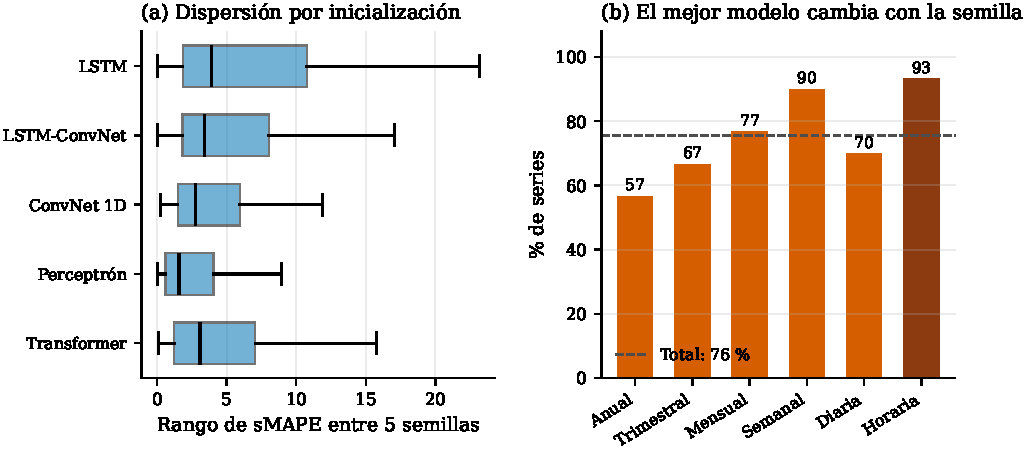
\includegraphics[width=\linewidth]{figuras/fig8_varianza_semillas.pdf}
\caption{(a) Distribución del rango de sMAPE entre cinco semillas, por arquitectura.
(b) Porcentaje de series en las que la arquitectura ganadora cambia al variar la
semilla. La frecuencia horaria, destacada, es la más inestable de las seis pese a ser
la única donde las redes superan al benchmark.}
\label{fig:semillas}
\end{figure}

\begin{table}[htbp]
\centering
\caption{Estabilidad del ranking por frecuencia. La brecha es la diferencia de sMAPE
entre la mejor y la segunda arquitectura; el ruido es el rango mediano entre semillas.}
\label{tab:estabilidad}
\begin{tabular}{lrrrr}
\toprule
\textbf{Frecuencia} & \textbf{Cambia el ganador} & \textbf{Brecha 1\textordmasculine--2\textordmasculine} & \textbf{Ruido} & \textbf{Ruido/brecha} \\
\midrule
Horaria     & \textbf{93\,\%} & 0.41 & 2.25 & \textbf{5.5$\times$} \\
Semanal     & 90\,\% & 1.02 & 4.85 & 4.8$\times$ \\
Mensual     & 77\,\% & 0.94 & 2.68 & 2.8$\times$ \\
Diaria      & 70\,\% & 0.40 & 1.01 & 2.5$\times$ \\
Trimestral  & 67\,\% & 1.61 & 3.87 & 2.4$\times$ \\
Anual       & 57\,\% & 2.48 & 4.27 & 1.7$\times$ \\
\midrule
Total       & 76\,\% & 0.92 & 2.81 & 3.0$\times$ \\
\bottomrule
\end{tabular}
\end{table}

\paragraph{La inestabilidad es máxima donde las redes funcionan.} El
Cuadro~\ref{tab:estabilidad} contiene el resultado más incómodo del trabajo. La
frecuencia horaria es la única donde las arquitecturas neuronales superan al
benchmark (Sección~\ref{sec:horaria}, OWA entre $0.76$ y $0.81$), y es también \emph{la más
inestable de las seis}: el ganador cambia en el 93\,\% de las series y el ruido de
inicialización quintuplica la brecha entre el primero y el segundo.

La consecuencia es precisa. En series horarias puede sostenerse que \emph{la familia}
de modelos neuronales es competitiva, pero no \emph{cuál arquitectura} lo es. Un
trabajo que reporte, a partir de una sola corrida, que una arquitectura supera a otra
en datos horarios está reportando ruido de inicialización con alta probabilidad.

El patrón por frecuencia no responde al tamaño muestral sino a la separación entre
arquitecturas: las frecuencias donde la brecha entre la primera y la segunda es
pequeña ---horaria $0.41$, diaria $0.40$, mensual $0.94$--- son aquellas donde la
elección del ganador es más frágil, con independencia de cuántas observaciones tenga
cada serie.

\paragraph{Promediar semillas no resuelve la selección.}\label{sec:ensamble}
La respuesta habitual a la inestabilidad por inicialización es promediar varias
semillas. Conviene distinguir dos objetivos que esa práctica persigue, porque solo uno
se resuelve así.

Promediar \emph{pronósticos} reduce el error, y es la razón clásica para construir
ensambles; ese efecto no se cuantifica aquí, porque el experimento registró los errores
por semilla y no las predicciones. Promediar \emph{puntajes} para decidir qué
arquitectura usar es un objetivo distinto, y ese sí se midió.

Se comparó la arquitectura ganadora que arrojaría un experimento con $k$ semillas contra
la que arrojaría otro experimento independiente con $k$ semillas distintas. Con una sola
semilla, dos experimentos coinciden en el 52.6\,\% de los casos (1.800 comparaciones).
Con dos semillas promediadas, en el 60.8\,\% (2.700 comparaciones). La mejora es de
ocho puntos y el resultado sigue siendo próximo al azar.

La razón es de escala. El desvío del promedio decrece como $1/\sqrt{k}$, pero parte de
1.18 puntos de sMAPE, mientras que la brecha mediana entre la primera y la segunda
arquitectura es de 0.92 puntos. Con cinco semillas, la diferencia esperable entre dos
experimentos independientes es todavía el 80\,\% de esa brecha. Alcanzar un ruido igual
a la mitad de la brecha exigiría del orden de trece semillas por serie y arquitectura.

La conclusión operativa no es que los ensambles sean inútiles ---reducen el error del
pronóstico, que es un beneficio real y no medido aquí--- sino que \textbf{con un
presupuesto realista de inicializaciones, la mejor arquitectura para una serie dada no
es identificable}. Ante eso caben dos posturas defendibles: combinar arquitecturas en
lugar de elegir una, o elegir la más estable ---el perceptrón, con un coeficiente de
variación de 6.2\,\%--- y aceptar los 0.33 puntos de sMAPE que cede frente al
Transformer.

\paragraph{Fijar la semilla no basta para reproducir.} Las tres frecuencias del
experimento preliminar se reejecutaron con las mismas series y las mismas semillas,
esperando reproducción exacta. \textbf{Ninguna de las 2.250 mediciones compartidas se
repite}; la diferencia máxima en sMAPE alcanza $105.8$. La causa no es la semilla sino
el entorno: la corrida preliminar empleó cuatro hilos de cómputo y la definitiva dos,
y sin habilitar determinismo a nivel de operación el orden de reducción en punto
flotante depende del número de hilos.

El estadístico agregado, en cambio, sí se reproduce: el porcentaje de series en las
que cambia el ganador pasa de 68\,\% a 67\,\% sobre las mismas tres frecuencias. Un
punto de diferencia. \emph{Ninguna medición individual sobrevive a la reejecución; la
conclusión sí.}

Esto refuerza el argumento en lugar de debilitarlo y agrega una recomendación al
protocolo de reporte: informar la semilla es insuficiente, hay que declarar además el
número de hilos y la configuración de determinismo, y los resultados deben leerse como
estadísticos sobre muchas series y no como mediciones puntuales.


% =====================================================================
\section{Discusion}\label{sec:discusion}
% =====================================================================

\paragraph{De la correlación a la decisión.} La objeción natural a un índice descriptivo
es que correlacionar no es servir, y buena parte de la literatura de características de
series de tiempo no la responde. La Sección~\ref{sec:enrutamiento} la responde como
corresponde: con una regla aprendida sobre unas series y evaluada sobre otras. El aporte
es modesto en magnitud ---recorre el 10.5\,\% de la distancia hacia el óptimo
alcanzable--- pero consistente, significativo e incremental respecto del \emph{control
correcto}: cualquier trabajo que proponga un criterio de estratificación debería
compararse contra la frecuencia y no contra un modelo único, que es un rival demasiado
débil. El escalar tampoco agota el problema: la mejor política sobre los 29 atributos
recorre el 15.0\,\% (Sección~\ref{sec:meta}), de modo que el índice obtiene siete décimas
de lo que consigue el aparato completo con una fracción del costo de mantenerlo.

\paragraph{Estratificar antes de modelar.} El mecanismo es el que motivaba la hipótesis
inicial: la estructura interna de una serie, medida antes de ajustar cualquier modelo,
anticipa la dificultad del pronóstico. El factor de 3.29 entre cuartiles extremos y la
diferencia de 116\,\% entre grupos permiten asignar presupuesto computacional de forma
diferenciada, reservando los métodos costosos para donde pueden marcar diferencia. Que la
granularidad óptima del enrutamiento coincida con la cardinalidad hallada por criterios
geométricos ---aunque no con su frontera--- sugiere que la binariedad es una propiedad del
conjunto y no un artefacto del procedimiento.

\paragraph{La estratificacion debe ser intra-frecuencia.} La dependencia observada
---de $r=0.736$ a $r=0.019$--- implica que aplicar un único umbral de complejidad
sobre la colección agregada sería un error. El índice funciona como criterio de
estratificacion dentro de cada frecuencia, no entre ellas.

\paragraph{Una frecuencia sin estructura.} El caso diario sugiere una conclusión
más general: existen colecciones para las cuales la busqueda de un mejor modelo
tiene retorno nulo. La evidencia más fuerte en ese sentido no proviene de este
trabajo sino de la competencia misma: los resultados oficiales muestran que
\emph{tanto el método ganador como el segundo pierden contra Naive2 en las series
diarias} (Sección~\ref{sec:frecuencia}). Dos sistemas construidos por equipos
especializados, evaluados a ciegas, quedan por detrás de un paseo aleatorio
desestacionalizado en una frecuencia entera. Que el índice tampoco discrimine allí deja de
ser una debilidad y pasa a ser un diagnóstico correcto: detectarlo de antemano evita un
gasto que ningún método recuperará.

\paragraph{El techo, y de dónde viene.} El resultado más útil de este trabajo no es que el
índice funcione sino cuánto funciona, y frente a qué alternativa. La superioridad de la
combinación sobre la selección está establecida desde hace medio siglo
\cite{bates1969,wang2023} y no se reclama aquí; lo que estas páginas agregan es ponerla en
la misma escala que la caracterización estructural, sobre los mismos datos y protocolo. La
regla basada en el índice recorre el 10.5\,\% de la distancia hacia el oráculo por serie y
la mejor política sobre los 29 atributos el 15.0\,\%: el 85\,\% restante no lo alcanza
ninguno de los dos. \textbf{El límite no lo impone haber resumido la estructura en un
escalar: lo impone la selección de modelos por características como enfoque}, y quien
busque cerrar ese 85\,\% no lo hará refinando el vector de atributos. La
Sección~\ref{sec:m3} lo confirma fuera de M4, donde la fracción sin recorrer llega al
93.3\,\%.

La causa es identificable. El clasificador que predice \emph{cuál} modelo gana acierta
solo en el 18.5\,\% de las series (Sección~\ref{sec:meta}), y la arquitectura neuronal
ganadora cambia con la semilla en el 76\,\% de ellas (Sección~\ref{sec:semillas}): se
decide sobre una señal inestable, porque los candidatos están separados por menos que el
ruido de la propia medición. De ahí una recomendación de
diseño concreta: \textbf{conviene decidir sobre el error esperado de cada candidato y no
sobre cuál de ellos va a ganar}. La razón no es que la etiqueta sea ruido ---las dos
formulaciones comparten esa etiqueta--- sino que predecir el ganador y creerle descarta la
estructura de costos, y esa estructura es extrema: el 1\,\% peor de las series concentra
el 40\,\% del daño. Con la pérdida corregida y sin tocar nada más, el mismo clasificador
pasa de OWA 1.493 a 0.866 y se ubica por delante de la política de regresión (0.875).

\paragraph{Reproducibilidad de los rankings neuronales.} El resultado de la
Sección~\ref{sec:semillas} tiene alcance más allá de este trabajo: si en el 76\,\% de las
series la arquitectura ganadora depende de la semilla ---y en el 93\,\% en la frecuencia
donde esas arquitecturas efectivamente funcionan--- los rankings finos que no reportan
varianza entre inicializaciones no son interpretables.

A esto se suma que fijar la semilla resultó insuficiente para reproducir: al variar el
número de hilos de cómputo, ninguna de las 2.250 mediciones repetidas coincidió, pese a
que el estadístico agregado se mantuvo dentro de un punto porcentual. La recomendación
práctica es doble: declarar semilla, número de hilos y configuración de determinismo, y
reportar dispersión entre inicializaciones como parte del protocolo estándar. Una tercera
---promediar varias semillas--- resulta menos favorable de lo que suele suponerse
(Sección~\ref{sec:ensamble}).

\paragraph{Implicaciones para sistemas en producción.} La distinción entre fallo mediocre
y fallo catastrófico (Sección~\ref{sec:extremos}) es determinante para el despliegue: un
sistema que sirve pronósticos automáticos debería incorporar una cota de plausibilidad
---rechazar los que se alejen del rango histórico por encima de un múltiplo del rango
intercuartil--- antes de exponer el resultado.


% =====================================================================
\section{Limitaciones}\label{sec:limitaciones}
% =====================================================================

\begin{enumerate}
\item \textbf{Cobertura del vector de características.} 65 series semanales se
      descartan por longitud insuficiente, de modo que los análisis estructurales
      cubren 99{,}935 de 100{,}000 series. La pérdida se concentra en la frecuencia
      con menor tamaño muestral.

\item \textbf{Ordenes fijos en los modelos estadísticos.} ARIMA y SARIMA se ajustan
      con ordenes $(1,1,1)$ y $(1,1,1)(1,1,1)_m$ sin selección automática. La
      elección es deliberada ---se busca una medida homogenea de dificultad y no el
      mejor modelo por serie--- pero implica que los OWA reportados son cotas
      inferiores del desempeño alcanzable.

\item \textbf{Tamaño de la evaluación de modelos.} El banco se evaluó
      sobre 5{,}773 series y no sobre las 100{,}000, por costo computacional. Las
      muestras son aleatorias dentro de cada frecuencia, con estratificacion por
      categoría en la anual y la mensual. El desbalance importa donde se pondera por
      población: la frecuencia mensual pesa el 48\,\% de la colección y aporta
      1{,}000 series evaluadas de 48{,}000, el 2.1\,\%. Se comprobó qué cambiaría al
      corregirlo: anulando el error de muestreo de esa frecuencia en el bootstrap
      ---el límite de evaluarla completa--- el intervalo de la
      Sección~\ref{sec:nbeats} se estrecha de $0.023$ a $0.017$ y sigue conteniendo el
      cero: el desbalance es real pero no es lo que sostiene aquel empate. La frecuencia
      anual sí se amplió, de 1{,}000 a 2{,}000 series, por ser la que más aportaba a la
      incertidumbre entre políticas; el efecto fue estrechar los intervalos sin alterar
      ningún veredicto, salvo hacer visible que la diferencia entre combinar y
      estratificar nunca había sido significativa.

\item \textbf{Alcance del experimento de semillas.} La varianza por inicialización
      se midió sobre 180 series, 30 de cada frecuencia. El resultado cualitativo
      ---el ganador cambia--- se reprodujo en una reejecución independiente con una
      diferencia de un punto porcentual, pero los porcentajes exactos conllevan la
      incertidumbre de esa muestra.

\item \textbf{Periodo estacional en la frecuencia trimestral.} La configuración
      registrada revela que ARIMA y SARIMA se ajustaron sobre las series trimestrales
      con $m=12$ en lugar de $m=4$, por un parámetro que no se propagó. Sobre una
      submuestra de 50 series el sMAPE medio pasa de $9.231$ a $9.421$, la selección
      automática de órdenes produce el mismo modelo en 23 de las 50 y la diferencia no
      es significativa (Wilcoxon pareado, $p=0.97$). Se documenta por transparencia; las
      conclusiones no dependen de ello.

\item \textbf{Convenciones de estacionalidad.} Dos frecuencias se procesaron con $m=12$
      en la construcción de rezagos antes de alinear el pipeline con la definición
      oficial de M4. Los resultados estructurales no dependen de esa elección; los
      errores de pronóstico almacenados para esas frecuencias la arrastran.

\item \textbf{Marco muestral.} Un archivo intermedio de la frecuencia mensual quedó
      truncado en $2^{14}$ series de 48{,}000 y, como M4 ordena por categoría económica,
      ese bloque contenía sólo dos de las seis. El muestreo se rehízo de forma
      estratificada; se documenta porque el sorteo era correcto y el sesgo provenía del
      marco, sin señal de alarma observable en el procedimiento.

\item \textbf{El banco de modelos precede a las arquitecturas neuronales
      recientes.} Las cuatro redes evaluadas ---perceptrón, ConvNet 1D, LSTM y
      Transformer--- son arquitecturas genéricas entrenadas serie por serie, y no hay
      modelos globales diseñados para colecciones, como N-BEATS \cite{oreshkin2020}. La
      afirmación de que solo seis modelos superan al benchmark está condicionada a este
      banco, y uno actualizado modificaría qué modelos componen los conjuntos de la
      Sección~\ref{sec:combinar}. No cambiaría la comparación entre políticas, porque
      todas operan sobre el mismo banco.

\item \textbf{N-BEATS no converge en la frecuencia mensual.} Con la implementación
      empleada, el modelo falla de forma sistemática en mensual (sMAPE mediano 31.3
      frente a 14.4 del benchmark, en las cinco semillas). El fallo es del centro de la
      distribución y no de la cola: no son casos extremos sino un modelo que no aprende.
      Como mensual concentra el 48\,\% de la colección, no se reporta ningún OWA global
      de N-BEATS. El efecto sobre la Sección~\ref{sec:nbeats} es conservador: con una
      implementación que funcionara en las seis frecuencias, la política óptima se
      acercaría aún más a «usar siempre el mismo modelo», que es la dirección en que ya
      apunta el resultado.

\item \textbf{Asimetría de datos de entrenamiento.} N-BEATS se entrena con todas las
      series de cada frecuencia mientras que los candidatos del banco se ajustan serie
      por serie sobre la muestra evaluada. No hay fuga ---sólo se usan los tramos de
      entrenamiento--- pero parte de su ventaja mide el acceso a dos órdenes de magnitud
      más de series y no sólo la arquitectura.

\item \textbf{Comparación indirecta con FFORMA.} La Sección~\ref{sec:meta}
      implementa el \emph{enfoque} de FFORMS y FFORMPP sobre estos datos, no los
      métodos publicados. FFORMA combina pronósticos con pesos aprendidos y el
      registro disponible conserva errores por serie, no las predicciones de su
      conjunto base; su OWA publicado corresponde además a otro conjunto de series
      y otro pool de métodos, de modo que no es directamente comparable con las
      cifras de este trabajo.

\item \textbf{Qué afirman las pruebas sobre particiones.} Varios contrastes de este
      trabajo ---Wilcoxon pareado en las Secciones~\ref{sec:enrutamiento},
      \ref{sec:dospasos} y en la comparación con catch22--- toman la partición como
      unidad. Treinta particiones de las mismas 5{,}674 series no son treinta muestras
      independientes, de modo que esos $p$ miden \textbf{consistencia al volver a dividir
      la muestra} y no significancia poblacional; leídos como lo segundo serían
      anticonservadores. Las afirmaciones centrales del trabajo ---el aporte del índice
      por tamaño de conjunto, la comparación entre combinar y estratificar, y el régimen
      de la Sección~\ref{sec:nbeats}--- se sostienen en cambio sobre remuestreo de series,
      que es la unidad correcta para generalizar. El contraste de Friedman de la
      Sección~\ref{sec:friedman} no está afectado: bloquea por serie.

\item \textbf{Validez externa: las magnitudes son de M4, los mecanismos no.} La
      Sección~\ref{sec:m3} repite el protocolo sobre M3 y el resultado hay que decirlo
      completo: el techo y el diagnóstico del clasificador se repiten ---allí la mejor
      política deja sin recuperar el 93.3\,\% del hueco---, pero \textbf{el 10.5\,\% que
      recorre el enrutamiento por índice cae al 1.9\,\%}, porque el banco de M3 es
      demasiado homogéneo para que haya algo que repartir. El umbral de dispersión donde
      el régimen se invierte no fue replicado en ninguna otra colección. Las magnitudes de
      este trabajo deben leerse entonces como una medición sobre M4 y su banco, no como
      constantes del problema; los mecanismos sí son independientes de la colección: que
      una etiqueta inestable no se puede aprender, que una pérdida con cola larga exige
      decidir sobre el costo esperado y no sobre la clase más probable, y que promediar
      cancela sesgos entre componentes comparables y arrastra al mejor cuando uno domina.
\end{enumerate}


% =====================================================================
\section{Conclusiones}\label{sec:conclusiones}
% =====================================================================

Este trabajo mostró que una medida de estructura calculable antes de ajustar cualquier
modelo no solo describe la dificultad del pronóstico: sirve para decidir. Asignar modelo
según frecuencia y estrato de complejidad supera a asignarlo solo por frecuencia en las 30
particiones evaluadas fuera de muestra, y la granularidad óptima ---dos estratos--- es la
cardinalidad que el análisis de conglomerados había identificado por criterios internos,
sin observar ningún error de pronóstico. Dos caminos independientes llegan a que la
estructura explotable es binaria; no a la misma frontera, porque las dos particiones
concuerdan en el 70.1\,\% de las series.

El aporte central, sin embargo, no es ese sino su medida y su ubicación. La regla recorre
el 10.5\,\% de la distancia hacia el oráculo por serie y la mejor política sobre los 29
atributos el 15.0\,\%: veintinueve atributos compran diecisiete milésimas de OWA sobre un
escalar con dos estratos y dejan intacto el 85\,\% del hueco. \textbf{El techo no lo impone
el resumen escalar.} Sí lo impone en parte la decisión de \emph{elegir}: promediar los
cinco mejores de cada estrato amplía el recorrido de 8.5\,\% a 14.4\,\%, y esa decisión
pesa tanto como la de estratificar. Que combinar supere a elegir no es un hallazgo de este
trabajo sino de medio siglo de literatura \cite{bates1969,wang2023}; sí lo es medir ambas
decisiones en la misma escala, y constatar que saber \emph{qué} combinar vale 0.39 puntos
de OWA frente a sortear entre los diez mejores.

Ese resultado tiene un alcance que el trabajo delimita en lugar de dejar implícito. Al
incorporar al banco un modelo global moderno el régimen se invierte allí donde ese modelo
domina: en las cuatro frecuencias en que N-BEATS aventaja al segundo por entre 0.060 y
0.231 de OWA, elegir uno supera a combinar cinco y el aporte del índice deja de ser
significativo. Que la inversión no llegue al agregado depende de que la frecuencia
mensual, el 48\,\% de la colección, sea donde la implementación empleada no converge. Un
mismo mecanismo explica los dos regímenes ---promediar cancela sesgos entre iguales y
arrastra al mejor cuando uno domina---, de donde se sigue la recomendación operativa:
\textbf{mirar la dispersión de calidad del pool antes de decidir entre elegir y combinar}.
Dentro del régimen sin modelo dominante, el aporte del índice es máximo al elegir y decae
al combinar hasta no detectarse con tres o más: la caracterización sirve justamente en la
decisión que menos rinde. Es la tensión que el trabajo deja planteada, y reconcilia el
techo medido con el segundo puesto de FFORMA ---que combina en vez de elegir, de modo que
su mérito recae sobre los pesos aprendidos más que sobre las características--- en lugar
de contradecirlo.

La causa del techo quedó identificada, y corregida en el camino. La etiqueta que la
selección por características debe aprender ---cuál método gana en esta serie--- es en
buena medida ruido: en el 76\,\% de las series la arquitectura neuronal ganadora cambia
únicamente al variar la inicialización, con un máximo de 93\,\% en la frecuencia horaria.
Pero el fracaso del clasificador, que termina peor que no enrutar, \emph{no} es
consecuencia de ese ruido: con la misma etiqueta y el mismo bosque, cambiar la regla de
decisión de la clase más probable al mínimo arrepentimiento esperado lo lleva de OWA
$1.493$ a $0.866$. La recomendación de diseño se sostiene ---predecir el error de cada
candidato antes que predecir cuál gana--- pero por codificar la pérdida y no por esquivar
una etiqueta ruidosa. La acompaña una recomendación de reporte: los rankings finos entre
arquitecturas que no informan dispersión entre semillas no son interpretables.

La réplica sobre M3, con los pronósticos publicados de 22 métodos y el índice transferido
sin reajuste, separa lo que es del enfoque de lo que es de M4. El techo se sostiene y
empeora ---allí queda sin recuperar el 93.3\,\%--- y el diagnóstico del clasificador se
repite, incluso en un banco donde ningún candidato diverge. El margen del enrutamiento por
índice, en cambio, cae del 10.5\,\% al 1.9\,\%, porque cinco de los 22 métodos quedan a
menos del 5\,\% del mejor: es la heterogeneidad del banco, y no la de las series, la que
fija cuánto hay para repartir. El índice ordena por dificultad en las dos colecciones; sólo
en una de ellas eso se traduce en una mejor elección de modelo.

La medida que hace posible todo lo anterior es un índice de complejidad estructural sobre
29 descriptores de las 100{,}000 series: correlaciona con el error del pronóstico ingenuo,
separa cuartiles cuyo error medio difiere por un factor de 3.29 y no es redundante con las
medidas establecidas. Su poder discriminante depende con fuerza de la frecuencia, lo que
obliga a estratificar dentro de cada una. La diaria es el caso límite instructivo: ninguna
medida discrimina y, de manera consistente, ningún modelo supera al benchmark ---tampoco
los dos primeros de la competencia---. Un índice sin poder discriminante en una colección
es información accionable, no un fracaso del diagnóstico. El banco bajo la métrica oficial
confirma además que los métodos clásicos siguen siendo competitivos ---solo seis superan a
Naive2, el mejor con OWA $=0.936$--- y revela la inversión completa del orden en la
frecuencia horaria; el contraste de Friedman con post-hoc de Nemenyi matiza el ranking:
empate estadístico entre ARIMA, SARIMA y ETS en la cima, e híbridos cuyo problema no es el
desempeño típico sino el riesgo de cola.

La hipótesis de partida ---agrupar las series por estructura y asignar a cada grupo el
método que le corresponde--- resulta entonces correcta en su dirección, modesta en su
alcance y equivocada en su forma: la partición que la estructura admite es binaria y no
una taxonomía de regímenes, su aporte se concentra en la decisión que menos rinde, y su
magnitud depende del banco contra el que se la mida. Aun así, el grueso de la distancia
hacia el oráculo queda sin recorrer ---una distancia que acota por arriba lo recuperable y
no lo mide, porque incluye error que ningún modelo del banco podía evitar.

\paragraph{Trabajo futuro.} Tres líneas se desprenden: incorporar el índice como
variable de decisión en un sistema de selección automática y medir la ganancia frente a
una política uniforme; extender la evaluación a la colección completa; y, puesto que la
réplica sobre M3 mostró que el margen del enrutamiento depende de la heterogeneidad del
banco, medir esa dependencia de forma directa ---variando la composición del banco a
colección fija--- en lugar de seguir cambiando de colección.


% =====================================================================
\section*{Disponibilidad de código y datos}
% =====================================================================

Los datos provienen de la competencia M4 y son de acceso público \cite{m4results}; los de
la réplica externa, de los pronósticos publicados de M3 \cite{mcomp}. El código completo
---características, reducción, clustering, entropías, métricas oficiales, evaluación del
banco y los experimentos de enrutamiento, meta-aprendizaje, combinación y validación
externa--- está en \url{https://github.com/JorgeChiles/m4-estructura-combinacion}, bajo
licencia MIT, con las instrucciones de ejecución en orden y las dependencias con versiones
fijas. La reejecución de las etapas deterministas reproduce todo de forma exacta:
diferencia $0.00$ en el índice de las 99{,}935 series, en las asignaciones de grupo, en las
componentes principales, en las tres entropías y en los errores de los métodos
estadísticos y de aprendizaje automático. Los componentes estocásticos ---las redes--- no
reproducen, y esa falta de reproducibilidad se reporta como resultado en la
Sección~\ref{sec:semillas} en lugar de omitirse.


% =====================================================================
{\scriptsize
\begin{thebibliography}{99}
\setlength{\itemsep}{0pt}\setlength{\parskip}{0pt}
% =====================================================================

\bibitem{bates1969}
Bates, J. M., \& Granger, C. W. J. (1969). The combination of forecasts.
\emph{Operational Research Quarterly}, 20(4), 451--468.

\bibitem{wang2023}
Wang, X., Hyndman, R. J., Li, F., \& Kang, Y. (2023). Forecast combinations: an over
50-year review. \emph{International Journal of Forecasting}, 39(4), 1518--1547.

\bibitem{makridakis2020}
Makridakis, S., Spiliotis, E., \& Assimakopoulos, V. (2020).
The M4 Competition: 100,000 time series and 61 forecasting methods.
\emph{International Journal of Forecasting}, 36(1), 54--74.

\bibitem{makridakis2000}
Makridakis, S., \& Hibon, M. (2000). The M3-Competition: results, conclusions and
implications. \emph{International Journal of Forecasting}, 16(4), 451--476.

\bibitem{mcomp}
Hyndman, R. J. (2018). \emph{Mcomp: Data from the M-Competitions} [paquete de R,
versión 2.8]. Incluye las 3.003 series de M3 y los pronósticos de todos los métodos
participantes. \url{https://CRAN.R-project.org/package=Mcomp}

\bibitem{m4results}
M4 Team (2018). \emph{Evaluation and Ranks} [planilla de resultados oficiales de
la competencia M4]. Repositorio Mcompetitions/M4-methods.
\url{https://github.com/Mcompetitions/M4-methods}

\bibitem{smyl2020}
Smyl, S. (2020). A hybrid method of exponential smoothing and recurrent neural
networks for time series forecasting.
\emph{International Journal of Forecasting}, 36(1), 75--85.

\bibitem{wang2006}
Wang, X., Smith, K., \& Hyndman, R. (2006).
Characteristic-based clustering for time series data.
\emph{Data Mining and Knowledge Discovery}, 13(3), 335--364.

\bibitem{kang2017}
Kang, Y., Hyndman, R. J., \& Smith-Miles, K. (2017). Visualising forecasting algorithm
performance using time series instance spaces.
\emph{International Journal of Forecasting}, 33(2), 345--358.

\bibitem{fulcher2017}
Fulcher, B. D., \& Jones, N. S. (2017). hctsa: A computational framework for
automated time-series phenotyping using massive feature extraction.
\emph{Cell Systems}, 5(5), 527--531.

\bibitem{talagala2018}
Talagala, T. S., Hyndman, R. J., \& Athanasopoulos, G. (2023). Meta-learning how to
forecast time series. \emph{Journal of Forecasting}, 42(6), 1476--1501.

\bibitem{monteromanso2020}
Montero-Manso, P., Athanasopoulos, G., Hyndman, R. J., \& Talagala, T. S. (2020).
FFORMA: Feature-based forecast model averaging.
\emph{International Journal of Forecasting}, 36(1), 86--92.

\bibitem{oreshkin2020}
Oreshkin, B. N., Carpov, D., Chapados, N., \& Bengio, Y. (2020). N-BEATS: Neural basis
expansion analysis for interpretable time series forecasting.
\emph{International Conference on Learning Representations (ICLR)}.

\bibitem{lubba2019}
Lubba, C. H., Sethi, S. S., Knaute, P., Schultz, S. R., Fulcher, B. D., \& Jones, N. S.
(2019). catch22: CAnonical Time-series CHaracteristics.
\emph{Data Mining and Knowledge Discovery}, 33(6), 1821--1852.

\bibitem{bandt2002}
Bandt, C., \& Pompe, B. (2002). Permutation entropy: a natural complexity measure
for time series. \emph{Physical Review Letters}, 88(17), 174102.

\bibitem{richman2000}
Richman, J. S., \& Moorman, J. R. (2000). Physiological time-series analysis using
approximate entropy and sample entropy.
\emph{American Journal of Physiology --- Heart and Circulatory Physiology},
278(6), H2039--H2049.

\bibitem{lempel1976}
Lempel, A., \& Ziv, J. (1976). On the complexity of finite sequences.
\emph{IEEE Transactions on Information Theory}, 22(1), 75--81.

\bibitem{demsar2006}
Dem\v{s}ar, J. (2006). Statistical comparisons of classifiers over multiple data
sets. \emph{Journal of Machine Learning Research}, 7, 1--30.

\bibitem{talagala2019}
Talagala, T. S., Li, F., \& Kang, Y. (2022). FFORMPP: Feature-based forecast model
performance prediction.
\emph{International Journal of Forecasting}, 38(3), 920--943.

\bibitem{vanzyl2023}
van Zyl, T. L. (2023). Late meta-learning fusion using representation learning for
time series forecasting. \emph{arXiv preprint}. DOI: 10.48550/arXiv.2303.11000

\bibitem{vaiciukynas2021}
Vaiciukynas, E., Danenas, P., Kontrimas, V., \& Butleris, R. (2021). Two-step
meta-learning for time-series forecasting ensemble. \emph{IEEE Access}, 9,
62687--62696.

\bibitem{abdallah2025}
Abdallah, M., Rossi, R. A., Mahadik, K., Kim, S., Zhao, H., \& Bagchi, S. (2025).
Evaluation-free time-series forecasting model selection via meta-learning.
\emph{ACM Transactions on Knowledge Discovery from Data}, 19(3), 64:1--64:41.

\bibitem{digangi2022}
Di Gangi, L. (2022). Sparse convex combinations of forecasting models by meta
learning. \emph{Expert Systems with Applications}, 200, 116938.

\bibitem{raubitzek2021}
Raubitzek, S., \& Neubauer, T. (2021). Combining measures of signal complexity and
machine learning for time series analysis: A review. \emph{Entropy}, 23(12), 1672.
DOI: 10.3390/e23121672

\bibitem{huang2019}
Huang, Y., \& Fu, Z. (2019). Enhanced time series predictability with well-defined
structures. \emph{Theoretical and Applied Climatology}, 138(1--2), 373--385.

\bibitem{manero2021}
Manero, J., \& Béjar, J. (2021). Forecastability measures that describe the
complexity of a site for deep learning wind predictions.
\emph{Supercomputing Frontiers and Innovations}, 8(1), 8--27.

\bibitem{kovantsev2020}
Kovantsev, A., \& Gladilin, P. (2020). Analysis of multivariate time series
predictability based on their features. \emph{IEEE International Conference on Data
Mining Workshops (ICDMW)}, 348--355.

\bibitem{gundersen2023}
Gundersen, O. E., Shamsaliei, S., Kj\ae{}rnli, H. S., \& Langseth, H. (2023). On reporting robust and
trustworthy conclusions from model comparison studies involving neural networks and
randomness. \emph{ACM Conference on Reproducibility and Replicability}, 37--61.

\bibitem{agathangelou2020}
Agathangelou, P., Trihinas, D., \& Katakis, I. (2020). A multi-factor analysis of
forecasting methods: A study on the M4 competition. \emph{Data}, 5(2), 41.
DOI: 10.3390/data5020041

\bibitem{ingel2020}
Ingel, A., Shahroudi, N., Kängsepp, M., Tättar, A., Komisarenko, V., \& Kull, M.
(2020). Correlated daily time series and forecasting in the M4 competition.
\emph{International Journal of Forecasting}, 36(1), 121--128.

\bibitem{hyndman2006}
Hyndman, R. J., \& Koehler, A. B. (2006).
Another look at measures of forecast accuracy.
\emph{International Journal of Forecasting}, 22(4), 679--688.

\end{thebibliography}
}
